%%%%%%%%%%%%%%%%%%%%%%% file template.tex %%%%%%%%%%%%%%%%%%%%%%%%%
%
% This is a general template file for the LaTeX package SVJour3
% for Springer journals.          Springer Heidelberg 2010/09/16
%
% Copy it to a new file with a new name and use it as the basis
% for your article. Delete % signs as needed.
%
% This template includes a few options for different layouts and
% content for various journals. Please consult a previous issue of
% your journal as needed.
%
%%%%%%%%%%%%%%%%%%%%%%%%%%%%%%%%%%%%%%%%%%%%%%%%%%%%%%%%%%%%%%%%%%%
%
% First comes an example EPS file -- just ignore it and
% proceed on the \documentclass line
% your LaTeX will extract the file if required
\begin{filecontents*}{example.eps}
%!PS-Adobe-3.0 EPSF-3.0
%%BoundingBox: 19 19 221 221
%%CreationDate: Mon Sep 29 1997
%%Creator: programmed by hand (JK)
%%EndComments
gsave
newpath
  20 20 moveto
  20 220 lineto
  220 220 lineto
  220 20 lineto
closepath
  2 setlinewidth
gsave
  .4 setgray fill
grestore
stroke
grestore
\end{filecontents*}

\RequirePackage{fix-cm}
\newcounter{chapter}
\documentclass[smallextended]{svjour3}
\smartqed




\usepackage[table]{xcolor}    % loads also »colortbl«
\usepackage{hyperref}
\usepackage[usenames,dvipsnames,table]{xcolor}
\usepackage{times}
\usepackage{graphicx}
\usepackage{latexsym}
\usepackage{xspace}
\usepackage[fleqn]{amsmath}
\usepackage{amssymb}
\usepackage{amsfonts}
\usepackage{algorithm}
\usepackage[noend]{algpseudocode}
\usepackage[numbers]{natbib}
\usepackage{notoccite}
\usepackage{fixltx2e}
\usepackage{framed}
\usepackage{tabularx}
\usepackage[margin=0.1cm]{subcaption}
\usepackage[inline]{enumitem}
\usepackage{footmisc}



\newcommand{\wat}{\textcolor{red}{ ({\Large ?}) }\xspace}
\newcommand{\PADSEP}{-7pt}
\newcommand{\sergey}[1]{\textcolor{magenta}{{\sc Sergey:} #1}\xspace}
\newcommand{\sam}[1]{\textcolor{green}{{\sc Samuel:} #1}\xspace}
\newcommand{\samuel}[1]{\textcolor{green}{{\sc Samuel:} #1}\xspace}
\newcommand{\tias}[1]{\textcolor{blue}{{\sc Tias:} #1}\xspace}
\newcommand{\luc}[1]{\textcolor{red}{{\sc Luc:} #1}\xspace}

\newcommand{\constraints}{\ensuremath{\mathcal{T}}\xspace}
\newcommand{\format}[1]{\textit{#1}\xspace}
\newcommand{\generategroups}{\format{SuperblockAssignments}}
\newcommand{\extractgroups}{\format{extractGroups}}
\newcommand{\extracttables}{\format{extractTables}}
\newcommand{\learnconstraints}{\format{LearnConstraints}}
\newcommand{\findassignment}{\format{Subassignments}}
\newcommand{\postprocess}{\format{pruneRedundant}}
\newcommand{\constrainttorder}{\format{templateOrder}}
\newcommand{\template}{\format{constraint template}}
\newcommand{\sname}{\format{TaCLe}}


\newcommand{\CName}{Syntax\xspace}
\newcommand{\CSignature}{Signature\xspace}
\newcommand{\CFunction}{Definition\xspace}
\newcommand{\dependencies}{\ensuremath{\mathcal{D}}\xspace}
\newcommand{\groups}{\ensuremath{\mathcal{B}}\xspace}
\newcommand{\blocks}{\ensuremath{\mathcal{B}}\xspace}

\newcommand{\range}[3]{\ensuremath{#1[#2,#3]}}
\newcommand{\rangeto}[2]{#1{:}#2}
\newcommand{\rangeall}{:}

\newcommand{\eccalc}[2]{\ensuremath{#1 = #2}}
\newcommand{\ecrank}[2]{\eccalc{#1}{\textit{RANK}(#2)}}
\newcommand{\ecfkey}[2]{\ensuremath{\textit{FOREIGNKEY}(#1,#2)}}
\newcommand{\ecalldiff}[1]{\ensuremath{\textit{ALLDIFFERENT}(#1)}}
\newcommand{\eclookupf}[4]{\ensuremath{\textit{LOOKUP}_{\textit{#4}}(#1, #2, #3)}}
\newcommand{\eclookup}[4]{\eccalc{#1}{\eclookupf{#2}{#3}{#4}{}}}
\newcommand{\eclookupprod}[5]{\eccalc{#1}{#2 \times \eclookupf{#3}{#4}{#5}{}}}
\newcommand{\eclookupfuzzy}[4]{\eccalc{#1}{\eclookupf{#2}{#3}{#4}{fuzzy}}}
\newcommand{\ecperm}[1]{\ensuremath{\textit{PERMUTATION}(#1)}}
\newcommand{\ecseries}[1]{\ensuremath{\textit{SERIES}(#1)}}
\newcommand{\ecprod}[3]{\eccalc{#1}{#2 \times #3}}
\newcommand{\ecdiv}[3]{\eccalc{#1}{{#2} / {#3}}}
\newcommand{\ecdiff}[3]{\eccalc{#1}{#2 - #3}}
\newcommand{\ectotal}[3]{\eccalc{#1}{\textit{PREV}(#1) + #2 - #3}}
\newcommand{\ecproj}[2]{\eccalc{#1}{\textit{PROJECT}(#2)}}
\newcommand{\ecaggc}[3]{\eccalc{#2}{\textit{#1\textsubscript{col}}(#3)}}
\newcommand{\ecaggr}[3]{\eccalc{#2}{\textit{#1\textsubscript{row}}(#3)}}
\newcommand{\ecsumc}[2]{\eccalc{#1}{\textit{SUM\textsubscript{col}}(#2)}}
\newcommand{\ecsumr}[2]{\eccalc{#1}{\textit{SUM\textsubscript{row}}(#2)}}
\newcommand{\ecaggif}[5]{\eccalc{#2}{\textit{#1IF}(#3, #4, #5)}}
\newcommand{\ecsumif}[4]{\eccalc{#1}{\textit{SUMIF}(#2, #3, #4)}}
\newcommand{\ecsumprod}[3]{\eccalc{#1}{\textit{SUMPRODUCT}(#2, #3)}}

\newcommand{\numeric}{\format{numeric}}
\newcommand{\textual}{\format{textual}}
\newcommand{\integer}{\format{integer}}
\newcommand{\discrete}{\format{discrete}}
\newcommand{\plength}{\format{length}}
\newcommand{\psize}{\format{size}}
\newcommand{\ptype}{\format{type}}
\newcommand{\ptable}{\format{table}}
\newcommand{\por}{\format{orientation}}
\newcommand{\prows}{\format{rows}}
\newcommand{\pcols}{\format{columns}}
\newcommand{\nat}{\mathcal{N}}

\newcommand{\sbs}{B}
\newcommand{\sbl}[1]{\ensuremath{\sbs_{\textit{#1}}}}
\newcommand{\ssbl}[1]{\ensuremath{\sbs'_{\textit{#1}}}}
\newcommand{\bsbl}[1]{\ensuremath{\mathbf{\sbs_{\textit{#1}}}}}



\renewcommand{\arraystretch}{1.5}




\begin{document}

\title{Learning constraints in spreadsheets and tabular data}
% see http://www.acm.org/binaries/content/assets/publications/article-templates/sig-alternate-sample.tex

\author{Samuel Kolb* \and Sergey Paramonov* \and Tias Guns \and Luc De Raedt}
\institute{KULeuven\\ {*} Shared first author}

\maketitle

\begin{abstract}
Spreadsheets, CSV (comma separated value) files and other tabular data representations are in wide use today.
However, writing, maintaining and identifying good formulas for tabular data and spreadsheets can be time consuming and error-prone.
In this work, we investigate the automatic learning of constraints (formulas and relations) in raw tabular data in an unsupervised way.
We represent common spreadsheet formulas and relations through predicates and expressions whose arguments must satisfy the inherent properties of the formula/relation. The challenge is to automatically infer the set of constraints that is present in the data, without user information or labeled examples. 
We propose a two-stage generate and test method where the first stage uses constraint solving techniques to efficiently reduce the number of candidates in a generic way, based on the predicate signatures. 
Our approach takes inspiration from inductive logic programming, constraint learning and constraint satisfaction.
We show that we are able to accurately discover constraints in spreadsheets from various sources.
\end{abstract}

\section{Introduction}
% relevance of formulas and spreadsheets
Millions of people across the world use spreadsheets every day.
The tabular representation of the data is often intuitive, and the programming of functions in individual cells is quickly learned.
However, large and complex sheets (possibly with multiple tables and relations between them) can be hard to handle.
Many end-users lack the understanding of the underlying structures and relations in such sheets and the data they contain.
This is especially the case when spreadsheets have been exported from other software such as Enterprise Resource Planning (ERP) systems.
In this case, often a comma-separated values (CSV) format is used meaning that all formulas are lost, including inter-sheet formulas and relations.
%This limited understanding is especially the case with spreadsheets exported from other software such as ERP packages. In this case,
Even in manually created spreadsheets, it can be challenging to be consistent and correct with formulas across all tables.
For example the influential Reinhart-Rogoff economical paper ``Growth in a Time of Debt'' \cite{growth_in_time_of_debt} had some of its claims contested~\cite{flaw_excel}, after an investigation of the used Excel sheets was shown to contain mistakes in formulae.

% why learn them
Such issues and mistakes could be overcome through the development of intelligent user-assisting tools. A core aspect of such tools would be the ability to automatically discover what constraints and formulae are present in a spreadsheet. This is the problem we study in this paper. There are multiple applications that could build on this, such as rediscovery of constraints when importing raw data, auto-suggestion of formula's during spreadsheet use, automatic auto-completion of rows or columns, and consistency and error checking.

% why difficult
In this paper,  we investigate whether machine learning and knowledge discovery techniques can be used to learn constraints (formulas and other relations) in spreadsheet data in an unsupervised way.
From a machine learning point of view this is an unconventional problem because the data is in tabular form, but the constraints we wish to learn can involve both rows and columns of the table. Being unsupervised there is no labeled information either, although for every possible function one can verify whether a certain input satisfies the definition.
%Unlike in other knowledge discovery tasks, such as pattern mining~\cite{}, there are many different types of formula and constraints we wish to discover, each with their own signature (number and properties of arguments) and definition.
From a data mining point of view, the data is relational on the one hand, since we can have multiple tables with relationships between them, but also of mixed textual and numeric types. More closely related is clausal discovery~\cite{claudien,lallouet}, learning CSP constraints \cite{Quacq,Conacq,modelseeker} and dependency discovery in databases \cite{savnik}. But an important difference remains that we want to learn constraints on both columns and rows over integer, floating point as well as textual data.
Our inspiration comes from work on program synthesis, in particular Flashfill \cite{flashfill}, where the definition of a function (over textual cells only) is learned in spreadsheet data from very few examples.


% Moved up
The question that we ask in this paper is: is it possible to learn the set of constraints present in a spreadsheet, from just flat tabular spreadsheet data? The main challenge is the number of possible constraints and combinations of rows and columns that need to be tried as input to the constraints.
To answer this challenge we propose a general-purpose method and system, named \sname (from: Tabular Constraint Learner, pronounced ``tackle''), for discovering row-wise and column-wise constraints.
%
% contribs
Our contributions are as follows:
\begin{itemize}
\item we define the tabular constraint learning problem, where the goal is to constraints that range over entire rows or columns in an unsupervised way;
\item we propose an effective 2-stage generate and test method where the first stage reasons only over properties of contiguous blocks of rows/columns, and the second stage continues to investigate individual rows and columns and their content;
\item furthermore, in the first stage we use a constraint solver to efficiently enumerate all combinations of maximally contiguous blocks compatible with the candidate constraint's argument; %, using backtracking search and forward checking;
\item experiments on different publicly available spreadsheets show that the system is able to extract constraints with high precision and recall. 
\end{itemize}

%It operates directly on (headerless) tables of a spreadsheet in an unsupervised setting, that is, it reasons on raw tabular data directly with no example constraint instantiations given. %, and discovers column- and row-wise constraints.
%We demonstrate the utility of our approach in an experimental evaluation.
%Moreover, we sketch additional application scenario's such as autocompletion and error detection.


This paper is organized as follows.
Section \ref{sec:related_work} presents a detailed discussion of the related work. Section \ref{sec:formalization} introduces concepts relevant to our approach and our problem statement.  Section \ref{sec:approach} presents our approach. Section \ref{sec:evaluation} presents the evaluation of the approach. Section \ref{sec:applications} shows how our system can be used for applications.  Section \ref{sec:conclusions} provides conclusions.

%Due to the complexity of numeric computations in spreadsheets, people often fail to grasp the properties of the data, which leads to the so called Spreadsheet risk\footnote{\url{https://en.wikipedia.org/wiki/Spreadsheet\#Spreadsheet_risk}} and even caused major flaw in the famous economics papers \cite{flaw_excel} and billion-losses in the financial industry \cite{spreadsheet_risk_loss}. Tabular constraint learning provides a potential cure by indicating learned constraint violations and suggest possible fixes.

% {\it
% \textbf{Motivation}:
% \begin{itemize}
%   \item USED -- File generated from model, model got lost, need to reconstruct
%   \item Constraint programming is hard - is Excel hard?
%   \item Avoid manual analysis, provide selection of constraints
%   \item SOMEWHAT USED --Error checking
%   \item Completion, gain speed and insights (Complicated constraints, also complicated to verify, too much output)
% \end{itemize}

% \textbf{Novelty:}
% \begin{itemize}
%   \item USED -- Unsupervised setting (contrary to flashfill, etc)
%   \item Numeric, different constraints (contrary to single textual function solution in flashfill, etc)
%   \item USED -- Data format (2D) -- data is no longer in rows like a classic ML or DM settings
%   \item USED -- Declarative, general / modular, stacking of constraint problems
% \end{itemize}
%}
\section{Related Work}\label{sec:related_work}
\sname combines ideas from several existing approaches and different fields of research.

First, it borrows techniques from logical and relational learning \cite{luc_book}, as it finds
constraints in multiple relations (or tables). Unlike typical logical and relational learning
approaches, it focuses on data in spreadsheets and constraints on columns or rows in the sheets.
Furthermore, it derives a set of simple ``atomic'' constraints rather than a set of rules that each consist of a conjunction of literals as in clausal discovery \cite{claudien,lallouet}. Nevertheless, several ideas from logical and relational learning
proved to be useful, such as the use of a canonical form, a refinement graph, and pruning for redundancy. It also connects with the logical generalization of given formulas in a spreadsheet \cite{Isakowitz}, where one abstracts present formulas by introducing parameters in the place of particular cell references. The key difference here is that we discover constraints (formulas) in the data, we do not have or use any prior information on the formulas in a spreadsheet.


Second, there exist a number of algorithms in the constraint programming community that induce constraints from one or more examples and questions. Two well-known approaches include ModelSeeker \cite{modelseeker} and Quacq \cite{Quacq}.
The former starts from a single example in the form of a vector of values and then exhaustively looks for the most specific constraints from a large constraint library that hold in the vector. To this aim, it cleverly enumerates different de-vectorized tables; for instance, if the initial vector was of dimension $1 \times 20$, it would consider rearrangements of size $2 \times 10$, $4 \times 5$, $5 \times 4$, $\dots$ and Modelseeker would then look for both column, row  and even diagonal constraints. Key differences are that we assume given spreadsheets with \textit{multiple} tables; and that ModelSeeker's constraints are restricted to integer values and often typical for constraint programming community, e.g. aimed at combinatorial optimization and scheduling. Conacq \cite{Conacq} acquires a conjunction of constraints using techniques inspired on Mitchell's version spaces to process examples; its successor Quacq uses active learning to query the user regarding satisfiability. Each of the examples/queries is processed for each constraint, hence an important issue is how fast the algorithm converges to the entire solution set (e.g. for Sudoku).
The focus is again on integer variables and typical combinatorial optimisation constraints. In a similar spirit the field of equation discovery \cite{equation_discovery} focuses, guided by  heuristics based on the structure of physical equations and unit measures, on the discovery of physical formulas over numbers and times series.
However, they focus specifically on noisy physical data and formulas, e.g. a single variable can take values from a series of measurements to get a regression parameter estimate or they apply specific data transformation such as numerical calculation of time and partial derivatives, i.e. the method works with approximations; the equation structures are heavily biased towards parameter estimation, while we focus on discovery of different types of spreadsheet constraints which is an exact constraint satisfaction problem.
\sergey{rewritten, Samuel, does it sound fine now?}
\tias{Last sentence too vague, what is specific about physical data? btw, it is supervised, e.g. input-output and we are general? Also, it is 'one' conjunction of functions, e.g. one equation, or not? Please rewrite more precisely}
%As the conjunction for typical constraint programming problems (such as Sudoku) can be quite large, a key problem is to cope with redundant constraints. As Modelseeker, these systems focus on the types of constraints in combinatorial optimization but unlike ModelSeeker and our approach, they do not assume the variables are organized in tabular form.


Third, our work borrows from the seminal work of Gulwani et al. \cite{flashfill} on program synthesis for tabular data, which is incorporated in Microsoft’s Excel. In FlashFill, the end-user might work on a table containing the surnames (column A) and names (column B) of politicians. The first row might contain the values A1 = ``Blair'' and B1 = ``Tony'', and the user might then enter in cell C1 the value ``T.B.''. At that point FlashFill generates a program that produces the output ``T.B.'' for the inputs ``Blair'' and ``Tony'', and also applies it to the other politicians (rows) in the table. While it might need an extra example to deal with names such as ``Van Rompuy'', ``Herman'' and determine whether it should output ``H.V.'' or ``H.V.R.'', FlashFill learns correct programs from very few examples. Flashfill has been extended to e.g. FlashExtract \cite{flashextract} to produce a set of tables starting from an unstructured document (a txt or HTML file) with a set of examples marked for extraction. However, unlike our approach, Flashfill requires the user to identify explicitly the desired inputs/outputs from the function as well as to provide explicitly some positive and sometimes also negative examples.  In contrast, our approach is unsupervised, although it would be interesting to study whether it could be improved through user interaction and through user examples.  Another interesting open issue (for all of these techniques with the exception of logical and relational learning) is how to deal with possibly incomplete or noisy data.

Fourth, also related to this line of research is the work on deriving constraints in databases such as functional and multi-valued dependencies \cite{savnik, Mannila-Raiha} although that line of research has focused on more specialized techniques for specific types of constraints. Many of of the discovery techniques rely on the database schema~\cite{flach_dependency_discovery}, which is not available in our case. Techniques that work directly on the data have been investigated for the discovery of functional dependencies between attributes~\cite{tane_dependency_discovery}. The constraints and formulas we wish to learn go beyond that, including arithmetic, conditional arithmetic and \textit{fuzzy} lookups, for example.

Finally, worth mentioning is BayesDB \cite{BayesDB} and Tabular \cite{tabular}, two recent probabilistic modeling languages that have been specifically designed for dealing with relational data in tabular form and that can, as FlashFill, also automatically fill out missing values in a table.  However, unlike the other mentioned approaches, it is based on an underlying probabilistic graphical model that performs probabilistic inference rather than identify ``hard'' constraints.


\begin{figure}[thb]

  \begin{subfigure}{1\textwidth}
  \begin{center}
    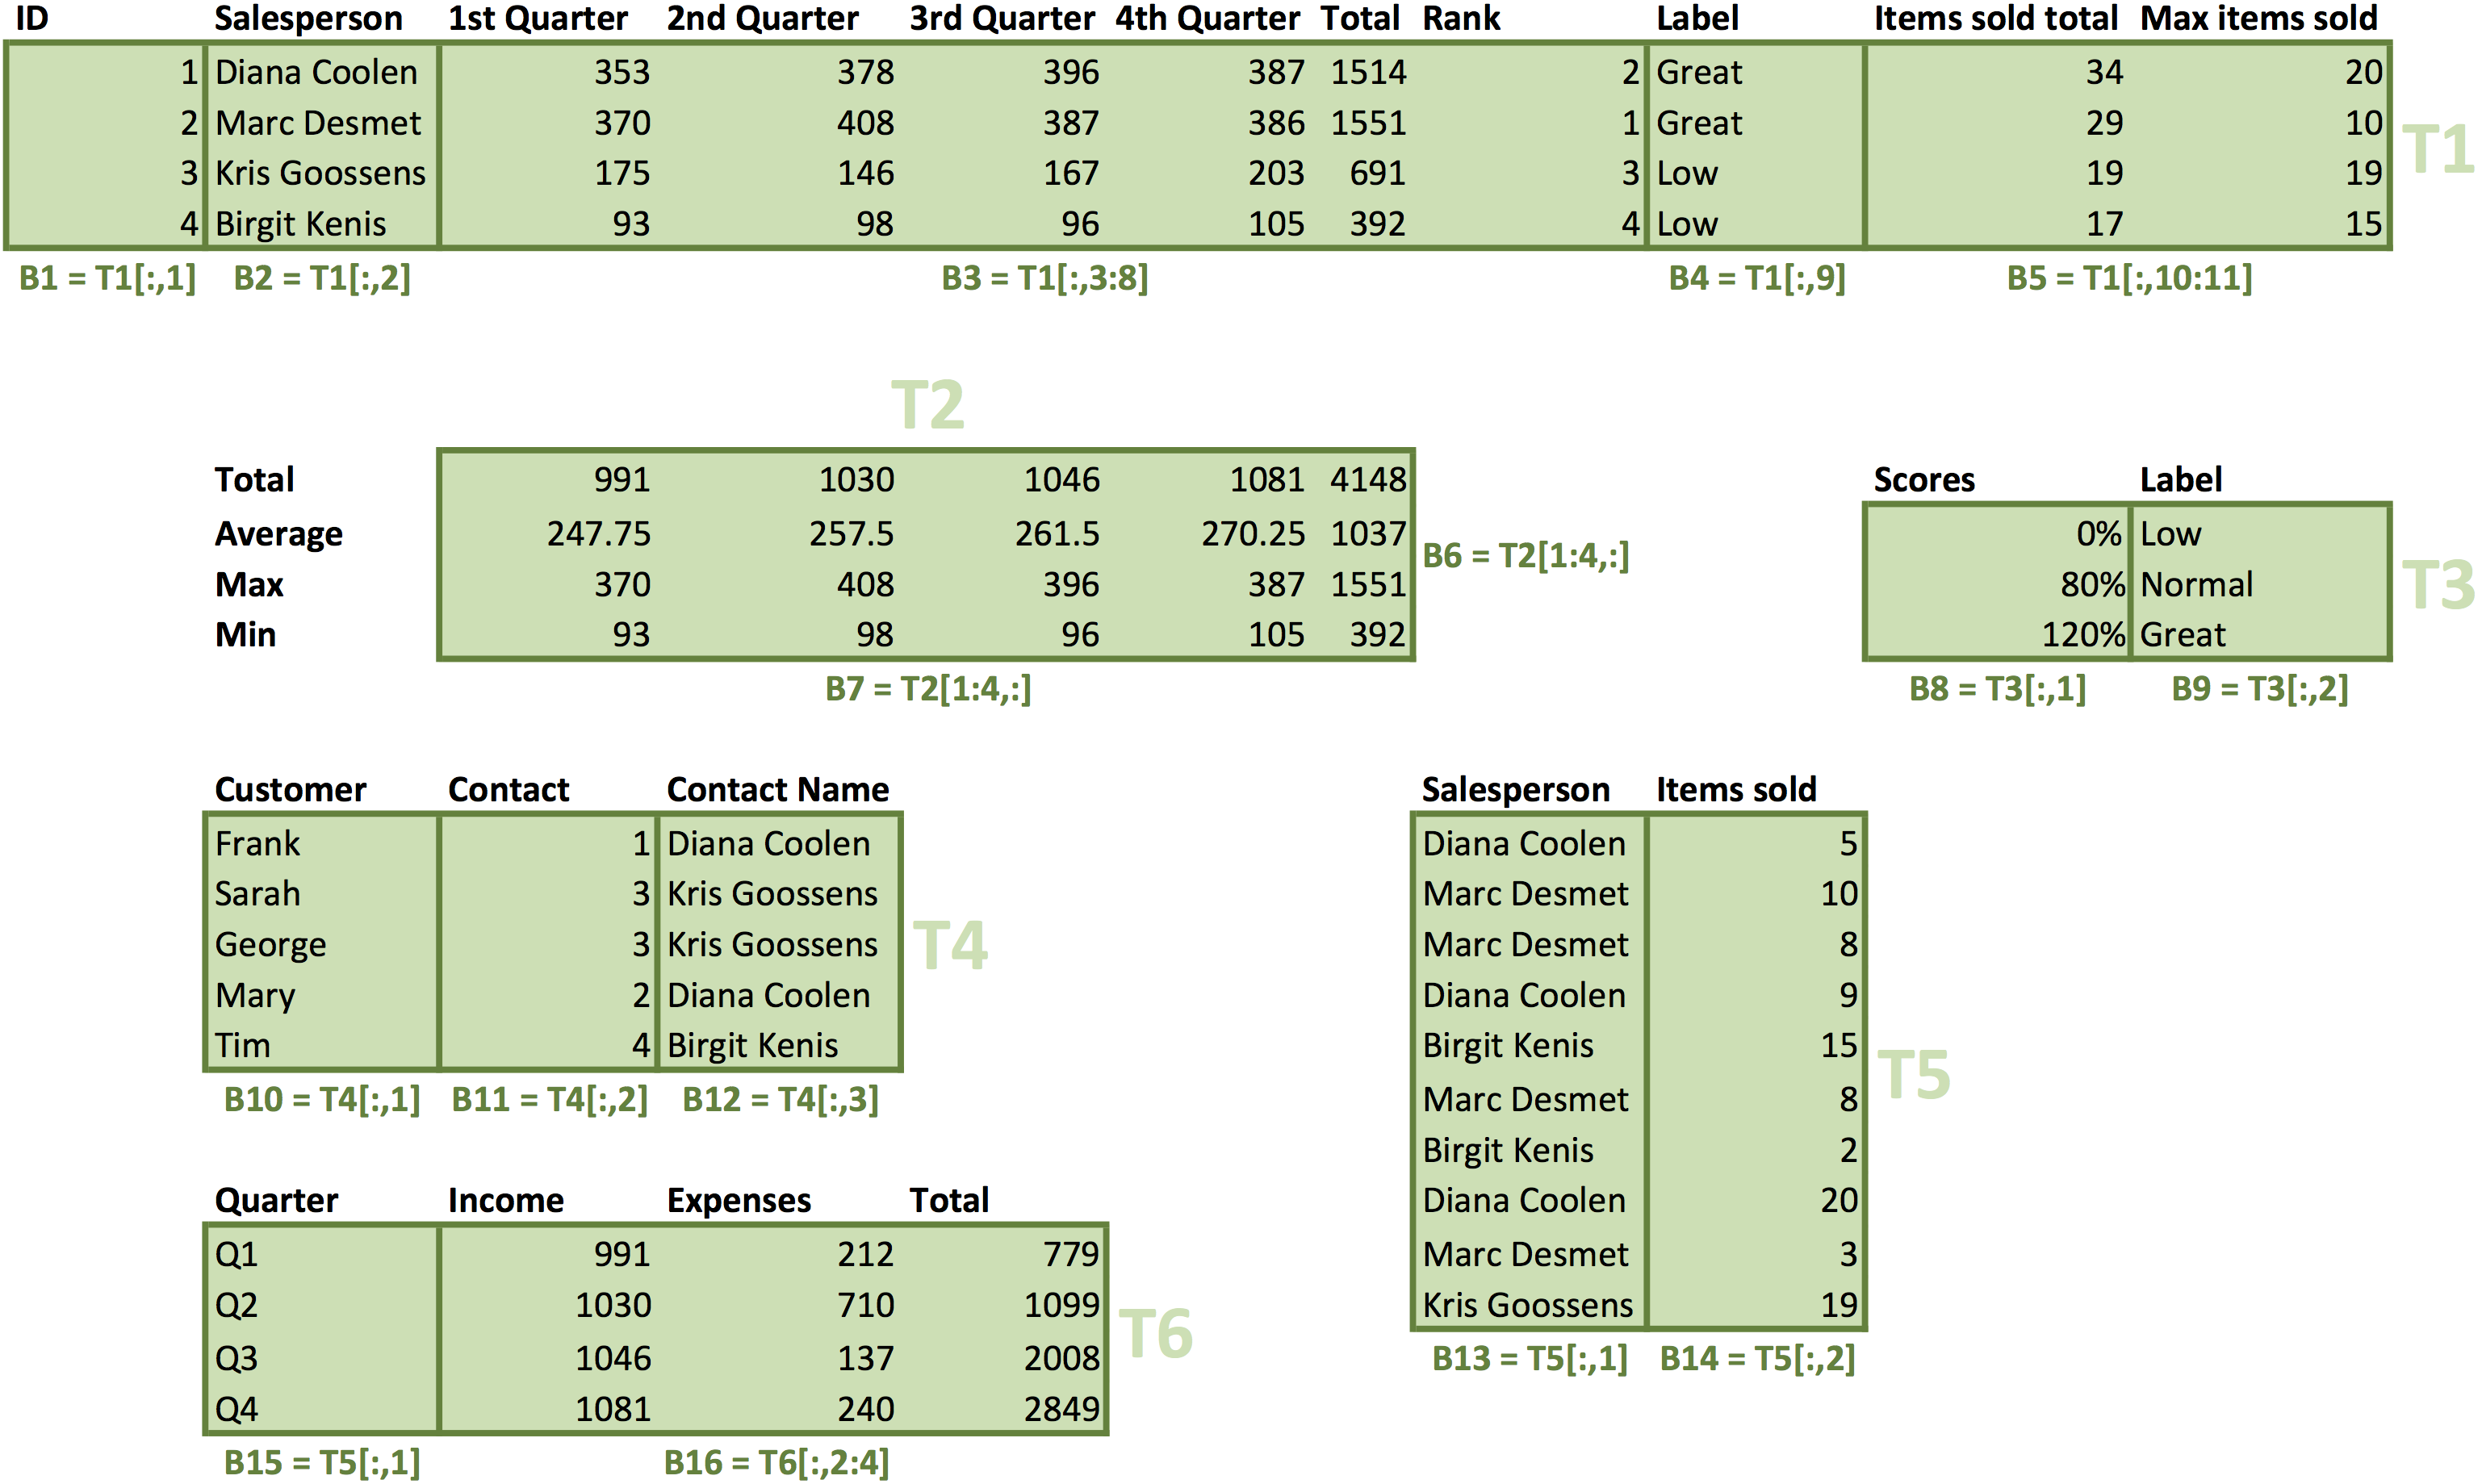
\includegraphics[width=1\textwidth]{figures/Demo2.png}
  \end{center}
  \vspace{-10pt}
  \caption{
    Example spreadsheet (black words and numbers only).
    Green background indicates headerless tables, dark borders indicate maximal type-consistent blocks.
    Most tables only contain type-consistent columns while table~$T_2$ also contains type-consistent rows (though its header indicates that it consists of row data).
%    However, due to the location of the header of~$T_2$ we can infer that it consists of row data.
    This example combines several Excel sheets based on exercise sessions in the book ``MS Excel 2010''~\cite{excel_book}.
    % I guess you want to save space by having everything in one figure, but it might be useful to have a smaller figure on the first page just to explain this example in a bit more detail (or use a smaller example here); it's quite overwhelming now}
  }
  \label{fig:main_example}
\end{subfigure}
\hfill
\begin{subfigure}{1\textwidth}
  {\scriptsize
    \begin{align*}
      % Table 1
%
%      &~\ecperm{\range{T_{1}}{\rangeall}{1}}, \ecperm{\range{T_{1}}{\rangeall}{8}} \\
%
      &~\ecseries{\range{T_{1}}{\rangeall}{1}}                                  && \ecsumc{\range{T_{2}}{1}{\rangeall}}{\range{T_{1}}{\rangeall}{\rangeto{3}{7}}} \\
      &~\ecrank{\range{T_{1}}{\rangeall}{1}}{\range{T_{1}}{\rangeall}{5}}^*     && \ecaggc{\textit{AVERAGE}}{\range{T_{2}}{2}{\rangeall}}{\range{T_{1}}{\rangeall}{\rangeto{3}{7}}}  \\
      &~\ecrank{\range{T_{1}}{\rangeall}{1}}{\range{T_{1}}{\rangeall}{6}}^*     && \ecaggc{\textit{MAX}}{\range{T_{2}}{3}{\rangeall}}{\range{T_{1}}{\rangeall}{\rangeto{3}{7}}} \\
      &~\ecrank{\range{T_{1}}{\rangeall}{1}}{\range{T_{1}}{\rangeall}{10}}^*    && \ecaggc{\textit{MIN}}{\range{T_{2}}{4}{\rangeall}}{\range{T_{1}}{\rangeall}{\rangeto{3}{7}}} \\
      &~\ecrank{\range{T_{1}}{\rangeall}{8}}{\range{T_{1}}{\rangeall}{7}}       && \ecsumc{\range{T_{4}}{\rangeall}{2}}{\range{T_{1}}{\rangeall}{\rangeto{3}{6}}} \\
      &~\ecrank{\range{T_{1}}{\rangeall}{8}}{\range{T_{1}}{\rangeall}{3}}^*     && \range{T_{4}}{\rangeall}{4} = PREV(\range{T_{4}}{\rangeall}{4}) + \range{T_{4}}{\rangeall}{2} - \range{T_{4}}{\rangeall}{3} \\
      &~\ecrank{\range{T_{1}}{\rangeall}{8}}{\range{T_{1}}{\rangeall}{4}}^*    && \eclookup{\range{T_{5}}{\rangeall}{2}}{\range{T_{5}}{\rangeall}{3}}{\range{T_{1}}{\rangeall}{2}}{\range{T_{1}}{\rangeall}{1}}^*\\
%
      &~\ecsumr{\range{T_{1}}{\rangeall}{7}}{\range{T_{1}}{\rangeall}{\rangeto{3}{6}}}   && \eclookup{\range{T_{5}}{\rangeall}{3}}{\range{T_{5}}{\rangeall}{2}}{\range{T_{1}}{\rangeall}{1}}{\range{T_{1}}{\rangeall}{2}} \\
%
      &~\ecaggif{\textit{SUM}}{\range{T_{1}}{\rangeall}{10}}{\range{T_{3}}{\rangeall}{1}}{\range{T_{1}}{\rangeall}{2}}{\range{T_{3}}{\rangeall}{2}}   && \ecaggif{\textit{MAX}}{\range{T_{1}}{\rangeall}{11}}{\range{T_{3}}{\rangeall}{1}}{\range{T_{1}}{\rangeall}{2}}{\range{T_{3}}{\rangeall}{2}} 
%
    % Table 2
%     &~\ecsumc{\range{T_{2}}{1}{\rangeall}}{\range{T_{1}}{\rangeall}{\rangeto{3}{7}}} \\
%
%     &~\ecaggc{\textit{AVERAGE}}{\range{T_{2}}{2}{\rangeall}}{\range{T_{1}}{\rangeall}{\rangeto{3}{7}}} \\
%
%     &~\ecaggc{\textit{MAX}}{\range{T_{2}}{3}{\rangeall}}{\range{T_{1}}{\rangeall}{\rangeto{3}{7}}},  \\
%
%     &~\ecaggc{\textit{MIN}}{\range{T_{2}}{4}{\rangeall}}{\range{T_{1}}{\rangeall}{\rangeto{3}{7}}} \\
%
    % Table 4
%     &~\ecsumc{\range{T_{4}}{\rangeall}{2}}{\range{T_{1}}{\rangeall}{\rangeto{3}{6}}} \\
%
%     &~\range{T_{4}}{\rangeall}{4} = PREV(\range{T_{4}}{\rangeall}{4}) + \range{T_{4}}{\rangeall}{2} - \range{T_{4}}{\rangeall}{3} \\
%
    % Table 5
%     &~\eclookup{\range{T_{5}}{\rangeall}{2}}{\range{T_{5}}{\rangeall}{3}}{\range{T_{1}}{\rangeall}{2}}{\range{T_{1}}{\rangeall}{1}}^* \\
%
%     &~\eclookup{\range{T_{5}}{\rangeall}{3}}{\range{T_{5}}{\rangeall}{2}}{\range{T_{1}}{\rangeall}{1}}{\range{T_{1}}{\rangeall}{2}}
    \end{align*}}
  \vspace{-10pt}
  \caption{Constraints learned for the tables above, except for \textit{ALLDIFFERENT} (18), \textit{PERMUTATION} (2) and \textit{FOREIGNKEY} (5) constraints.
  Constraints marked with $*$ were not present in the original spreadsheets.}
  \label{fig:sol_example}
\end{subfigure}
  \caption{Running example}
\end{figure}


\section{Formalization}\label{sec:formalization}
Our goal is to automatically learn the constraints present between rows and/or columns in a spreadsheet. This is applicable not just to data from spreadsheets, but to any data in tabular form, hence the name.

%An example spreadsheet with tables is given in Figure~\ref{fig:main_example}, we will use this as running example throughout the paper.

We first introduce some terminology and the concept of a \template, after which we define the problem and make some additional considerations.

\subsection{Terminology}
Spreadsheets and tabular data may conceptually consist of multiple tables, such as in Figure~\ref{fig:main_example}. Note that a table can contain a header; however, we wish to reason over entire rows and columns of data, and hence we will consider \textbf{headerless tables} only.

Formally, a (headerless) table is an $n \times m$ matrix. Each entry is called a \textit{cell}.
A cell has a {\bf type}, which can be numeric or textual. We further distinguish numeric types in subtypes: integer and float. We also consider \textit{None} as a special type when a cell is empty; \textit{None} is a subtype of all other types.

A row or a column is \textbf{type-consistent} if all cells in that row or column are of the same base type, i.e. numeric or textual.
We will use notation $T[a,{:}]$ to refer to the $a$-th row of table $T$ and similarly $T[{:},a]$ for the $a$-th column.
For example, in Figure~\ref{fig:main_example}, $T_1[:,1] = [1,2,3,4]$ and $T_3[1,:] = ['$Diana Coolen$', 5]$.
$T_3[1, :]$ is not type-consistent while $T_1[:, 1]$ is.
%We will write \textbf{vector} to refer to a single row or column when its orientation does not matter.

The most important concept is that of a \textbf{block}. 
\begin{definition}
A \textbf{block} has to satisfy three conditions: 1)~it contains only entire rows or entire columns of a single headerless table; 2)~it is contiguous; and 3)~it is type-consistent.
The rows or columns have to be contiguous in the original table meaning that they must visually form a block in the table; and each of the rows/columns has to be of the same type. 
If a block contains only rows we say it has \textit{row-orientation}, if only columns, \textit{column-orientation}. 
\end{definition}

In line with this definition, we can use the following notation to refer to blocks: $B = T[\rangeto{a}{b},:]$ for a row-oriented block containing rows $a$ to $b$ in table $T$; and similarly $B = T[{:},\rangeto{a}{b}]$ for a column-oriented block.
We will refer to the \textit{vectors} of a block when we wish to refer to its rows/columns independently of their orientation.


A block has the following properties:
\begin{itemize}
\item \textit{type}: a block is type-consistent, so it has one type
\item \textit{table}: the table that the block belongs to
\item \textit{orientation}: either row-oriented or column-oriented
\item \textit{size}: the number of vectors a block contains
\item \textit{length}: the length of its vectors; as all vectors are from the same table, they always have the same length.
\item \textit{rows}: the number of rows in the block
(in row-oriented blocks this is equivalent to the size)
\item \textit{columns}: the number of columns in the block (in row-oriented blocks this is equivalent to the length)
\end{itemize}

%We call a group $G$ \textit{numeric} (\textit{textual}, etc), written as \textit{numeric(G)}, if all its vectors contain numeric (textual, etc) elements.

%For notational convenience, we will refer to vectors in {\rm roman} and to groups in {\bf bold}. {\bf CHECK}

\begin{example}
Consider the (headerless) table~$T_1$ in Figure~\ref{fig:main_example}.
Its rows are not type consistent (i.e. they contain both numeric and textual data).
However, the table can be partitioned into five column-oriented blocks $\sbl{1}, \sbl{2}, \sbl{3}, \sbl{4}, \sbl{5}$, as shown in the figure ($\sbl{1} = \range{T_1}{\rangeall}{1}$, $\sbl{2} = \range{T_1}{\rangeall}{2}$, $\sbl{3} = \range{T_1}{\rangeall}{\rangeto{3}{8}}$, \dots).
\end{example}

\begin{definition}
\textbf{Block containment $\sqsubseteq$.} 
A block $B'$ is contained in a block $B$, $B' \sqsubseteq B$, iff both are valid blocks (contiguous, type consistent) with the same orientation and table, and each of the vectors in $B'$ is also in $B$. For row-oriented blocks: $B' \sqsubseteq B \Leftrightarrow B=\range{T}{\rangeto{a}{b}}{\rangeall} \wedge B'=\range{T}{\rangeto{a'}{b'}}{\rangeall} \wedge a \leq a' \wedge b' \leq b$ and similarly for column-oriented blocks.
\end{definition}

We will sometimes write that $B'$ is a \textit{subblock} of $B$ or that $B$ is a \textit{superblock} of $B'$.
%
An example of block containment is $T_1[:,\rangeto{3}{6}] \sqsubseteq T_1[:,\rangeto{3}{8}] $, which contains the sales numbers of all employees for the four quarters.


\begin{table}[htb]
\caption{
  Overview of constraint templates implemented in \sname.
  Subgroups in normal font have to be vectors, whereas subgroups in \textbf{bold} may contain more than one vector;
  $\discrete(x)$ is a shortcut for: $\textual(x) \lor \numeric(x)$.
  Templates marked with $*$ are \textit{structural}, i.e. they are not functional and cannot be implemented in most spreadsheet software.
  Templates marked with $\dagger$ are \textit{aggregate} templates, the table shows \textit{SUM} but \sname also supports \textit{MAX}, \textit{MIN}, \textit{AVERAGE}, \textit{PRODUCT} and \textit{COUNT}.
  %{\luc{maybe say s.th. about some fancy constraints: example of a more complex one in the text (what does conditional mean, aggregate ... )}}
}
\label{table:constraints}
\resizebox{1.0\columnwidth}{!}{%
  {\normalsize \centering
  \begin{tabularx}{1.70\textwidth}{l X X}
    \textbf{\CName} & \textbf{\CSignature} & \textbf{\CFunction}\\ \hline \hline
    $\ecalldiff{\sbl{x}}^*$
      & $\discrete(\sbl{x})$
      
      & All values in $\sbl{x}$ are different. $i \neq j$: $\sbl{x}[i] \neq \sbl{x}[j]$
      \\[\PADSEP] \hline

    $\ecperm{\sbl{x}}^*$
      & $\numeric(\sbl{x})$, $\ecalldiff{\sbl{x}}$
      
      & The values in $\sbl{x}$ are a permutation of the numbers $1$ through $\plength(\sbl{x})$.
      \\ \hline

    \ecseries{\sbl{x}}
      & $\integer(\sbl{x})$ and $\ecperm{\sbl{x}}$
      
      & $\sbl{x}[1] = 1$ and $\sbl{x}[i] = \sbl{x}[i - 1] + 1$.
      \\[\PADSEP] \hline

    $\ecfkey{\sbl{fk}}{\sbl{pk}}^*$
      & $\sbl{fk}$ and~$\sbl{pk}$ are $\discrete$; they must have different $\ptable$s but the same $\ptype$; and $\ecalldiff{\sbl{pk}}$

      & Every value in~$\sbl{fk}$ also exist in~$\sbl{pk}$ \\[\PADSEP] \hline

    \eclookup{\sbl{r}}{\sbl{fk}}{\sbl{pk}}{\sbl{val}}
      & $\sbl{fk}$ and $\sbl{pk}$ are $\discrete$; arguments $\{\sbl{fk}, \sbl{r}\}$ and $\{\sbl{pk}, \sbl{val}\}$ within the same set have the same \plength, \ptable and \por; $\sbl{r}$ and~$\sbl{val}$ have the same type; and \ecfkey{\sbl{fk}}{\sbl{pk}}.
      
      & $\sbl{r}[i] = \sbl{val}[j]$ where $\sbl{pk}[j] = \sbl{fk}[i]$
      \\[\PADSEP] \hline

    \eclookupfuzzy{\sbl{r}}{\sbl{fk}}{\sbl{pk}}{\sbl{val}}
      & \textit{Same as lookup}
      
      & $\sbl{r}[i] = \sbl{val}[j]$ where $\sbl{pk}[j] \leq \sbl{fk}[i]$, $j$~maximal
      \\[\PADSEP] \hline

    \eclookupprod{\sbl{r}}{\sbl{1}}{\sbl{fk}}{\sbl{pk}}{\sbl{val}}
      & Arguments $\{\sbl{r}, \sbl{1}, \sbl{fk}\}$ are $\numeric$, arguments $\{\sbl{pk}, \sbl{val}\}$ are $\discrete$ and within both sets all arguments have the same \plength, \ptable and \por; also \ecfkey{\sbl{fk}}{\sbl{pk}}.
      
      & $\sbl{r}[i] = \sbl{1}[i] \times \eclookupf{\sbl{fk}}{\sbl{pk}}{\sbl{val}}{}[i]$.
      \\[\PADSEP] \hline

    \ecprod{\sbl{r}}{\sbl{1}}{\sbl{2}}
      & Arguments $\{\sbl{r}, \sbl{1}, \sbl{2}\}$ are all $\numeric$ and have the same $\plength$
      
      & $\sbl{r}[i] = \sbl{1}[i] \times \sbl{2}[i]$.
      \\[\PADSEP] \hline

    \ecdiff{\sbl{r}}{\sbl{1}}{\sbl{2}}
      & Arguments $\{\sbl{r}, \sbl{1}, \sbl{2}\}$ are all $\numeric$ and have the same $\plength$ and $ \por$
      
      & $\sbl{r}[i] = \sbl{1}[i] - \sbl{2}[i]$.
      \\[\PADSEP] \hline

    $\eccalc{\sbl{r}}{\frac{\sbl{1} - \sbl{2}}{\sbl{2}}}$
      & \textit{Same as \ecdiff{\sbl{r}}{\sbl{1}}{\sbl{2}}}

      & $\sbl{r}[i] = (\sbl{1}[i] - \sbl{2}[i]) / \sbl{2}[i]$.
      \\[\PADSEP] \hline

    \ecproj{\sbl{r}}{\bsbl{x}}
      & Arguments $\{\sbl{r}, \bsbl{x}\}$ all have the same $\plength$, $\por$, $\ptable$ and $\ptype$; $\bsbl{x}$ contains at least~2 vectors; and $\sbl{r} = \textit{SUM}_{\por(\bsbl{x})}(\bsbl{x})$
      
      & At every position~$i$ in $1$ through $\plength(\sbl{r})$ there is exactly one vector~$v$ in $\bsbl{x}$ such that $v[i]$ is a non-blank value, then $v[i] = \sbl{r}[i]$.
      \\[\PADSEP] \hline

    \ecrank{\sbl{r}}{\sbl{x}}
      & $\integer(\sbl{r})$; $\numeric(\sbl{x})$; and $\plength(\sbl{r}) = \plength(\sbl{x})$
      
      & The values in $\sbl{r}$ represent the rank (from largest to smallest) of the values in $\sbl{x}$ (including ties)
      \\[\PADSEP] \hline

    \ectotal{\sbl{r}}{\sbl{pos}}{\sbl{neg}}
      & Arguments $\{\sbl{r}, \sbl{pos}, \sbl{neg}\}$ are all $\numeric$ and all have the same $\plength$, which is at least $2$
      
      & $\sbl{r}[i] = \sbl{r}[i - 1] + \sbl{pos}[i] - \sbl{neg}[i]$.
      \\[\PADSEP] \hline

    $\ecsumr{\sbl{r}}{\bsbl{x}}^\dagger$
      & $\sbl{r}$ and $\bsbl{x}$ are $\numeric$; $\pcols(\bsbl{x}) \geq 2$; and $\prows(\bsbl{x}) = \plength(\sbl{r})$
      
      & $\sbl{r}[i] = \sum_{j = 1}^{\pcols(\bsbl{x})} \textit{row}(i, \bsbl{x})[j]$
      \\[\PADSEP] \hline

    $\ecsumc{\sbl{r}}{\bsbl{x}}^\dagger$
      & $\sbl{r}$ and $\bsbl{x}$ are $\numeric$; $\prows(\bsbl{x}) \geq 2$; and $\pcols(\bsbl{x}) = \plength(\sbl{r})$
      
      & $\sbl{r}[i] = \sum_{j = 1}^{\prows(\bsbl{x})} \textit{column}(i, \bsbl{x})[j]$
      \\[\PADSEP] \hline

    $\ecsumif{\sbl{r}}{\sbl{fk}}{\sbl{pk}}{\sbl{val}}^\dagger$
      & $\sbl{fk}, \sbl{pk}$ are $\discrete$; $\sbl{r}, \sbl{val}$ are $\numeric$; within the sets $\{\sbl{val}, \sbl{fk}\}$ and $\{\sbl{pk}, \sbl{r}\}$ arguments have the same $\plength$ and $\por$; $\sbl{fk}$ and $\sbl{val}$ have the same $\ptable$; $\sbl{fk}$ and $\sbl{pk}$ must have different $\ptable$s but the same $\ptype$; and \ecalldiff{\sbl{pk}}
      
      & \[\sbl{r}[i] = \sum_{j=1}^{\plength(\sbl{val})} \begin{cases}
          \sbl{val}[j] & \text{if } \sbl{fk}[j] = \sbl{pk}[i] \\
          0 & \text{otherwise}
        \end{cases}
      \] \\[\PADSEP] \hline
      
    \ecsumprod{\sbl{r}}{\sbl{1}}{\sbl{2}}
      & Arguments $\{\sbl{r}, \sbl{1}, \sbl{2}\}$ are $\numeric$; $\plength(\sbl{1}) = \plength(\sbl{2}) \geq 2$; and $\prows(\sbl{r}) = \pcols(\sbl{r}) = 1$
      
      & $\sbl{r}[1] = \sum_{j = 1}^{\plength(\sbl{1})} \sbl{1}[j] \times \sbl{2}[j]$.
    \end{tabularx}
  } % centering small
} % resizebox

\end{table}

\newcommand{\sigc}{\ensuremath{\format{Sig}_s}}
\newcommand{\defc}{\ensuremath{\format{Def}_s}}

\subsection{Constraint templates}
The goal is to learn constraints over blocks in the data. The knowledge needed to learn a constraint is expressed through {\template}s.
%
A \template $s$ is a triple $t = \textit{(\CName, \CSignature, \CFunction)}$:
%Let us elaborate on this:
\begin{itemize}
\item
\textit{\CName}  specifies the syntactic form of the constraint $s(\sbl{1}, ...,\sbl{n})$, that is, the name of the template together
with $n$ abstract arguments $\sbl{i}$.
Thus, a constraint is viewed as a relation or predicate of arity $n$ in first order logic.
Note that a function $\sbl{r}=f(\sbl{1},...,\sbl{n})$ can be represented with the $(n{+}1)$-ary predicate $s_f(\sbl{r},\sbl{1},...,\sbl{n})$.
Each argument will have to be instantiated with a block.
% the list of its variables $v_1,\dots,v_n$.  In ILP terminology, it is known as vocabulary.

\item \textit{\CSignature} defines the requirements that the arguments of the predicate must satisfy.
This can concern properties of individual blocks as well as relations between properties of arguments, for example that the corresponding blocks must belong to the same table or have equal length.
In terms of logical and relational learning \cite{luc_book}, the \CSignature is known as the {\em bias} of the learner, it specifies when the arguments of a constraint are well-formed.
We can capture this bias for a template~$s$ using a predicate $\sigc$.
\item \textit{\CFunction} is the actual definition of the constraint that specifies when the constraint holds.
Given an assignment of blocks to its arguments, it can be used to verify whether the constraint is satisfied or not by the actual data present in the blocks. %holds, in practice this will be a function that can be called when
%the arguments are full instantiated to decide whether the constraint is satisfied or not.
In logical and relational learning this is known as the background knowledge.
We introduce the predicate \defc~to capture this background knowledge for a template~$s$.
\end{itemize}

\begin{example}
The constraint templates implemented in \sname are defined in Table~\ref{table:constraints}.
A non-trivial example is, for example, the constraint template for the row-based sum:

\begin{itemize}
  \item \CName: $\ecsumr{\sbl{r}}{\bsbl{x}}$, for arguments $\sbl{r}$ and $\bsbl{x}$.
  
  \item \CSignature: $\sbl{r}$ has to be a single vector ($\textit{size}=1$) while $\bsbl{x}$ can be a block ($\textit{size}>=1$), which can be derived from the use of a normal or \textbf{bold} font.
  Both blocks have to be numeric.
  This constraint is orientation-specific, so it requires that the number of rows in $\bsbl{x}$ equals the length of $\sbl{r}$.
  Moreover, we add to the bias that the number of columns to sum over is at least~$2$.
  
  \item \CFunction: each value in the vector $\sbl{r}$ is obtained by summing over the corresponding row in $\bsbl{x}$.
  %For example, $\sbl{r} = [12, 7]$ and $\bsbl{x}$ consists of columns: $[5, 15]$, $[7, -8]$.
\end{itemize}
\textit{SUM} is an aggregate constraint, and a similar constraint is available for aggregate operators \textit{MIN}, \textit{MAX}, \textit{AVERAGE}, \textit{PRODUCT} and \textit{COUNT}. The \textit{conditional} aggregate variant \textit{SUMIF} only ranges over those cells that satisfy a condition on a related cell in that table, e.g. for the spreadsheet in Figure~\ref{fig:main_example}: $\range{T_1}{\rangeall}{10}$ and the data in $T_5$ for matching salesperson names.
\end{example}


It is helpful to see the analogy of constraint templates with first order logic (FOL) and constraint satisfaction.
From a FOL perspective, a constraint of the form $\ecrank{\sbl{r}}{\sbl{x}}$ can be seen as a predicate $\textit{RANK}(\sbl{r}, \sbl{x})$ where \textit{RANK} is the name of the predicate and its arguments~$\sbl{r}$ and~$\sbl{x}$ are terms, which can be seen as either uninstantiated variables or as concrete values.
This also holds in our setting, where an instantiation of a variable corresponds to a concrete block.
For example, for the spreadsheet in Figure~\ref{fig:main_example}, when we write $\ecrank{\range{T_1}{\rangeall}{8}}{\range{T_1}{\rangeall}{7}}$, then the value of $\sbl{r}$ is the $8$th vector in $T_1$: $\sbl{r} = \range{T_1}{\rangeall}{8} = [2,1,3,4]$ and the value of $\sbl{x}$ is the $7$th vector: $\sbl{x} = \range{T_1}{\rangeall}{7} = [1514, 1551, 691, 392]$.

%When looking into constraints like \textit{$B$ = RANK($A$)}, it is helpful to see the analogy with both first order logic (FOL) and with constraint satisfaction problems.
%From a FOL perspective, the name of the constraint ($\mathit{RANK}$) is just the predicate, and the arguments $B$ and $A$ are the terms, which can be seen as either uninstantiated variables or as values (concrete groups with values).
%This also holds in our setting: when we write
%      $\ecrank{\range{T}{\rangeall}{8}}{\range{T}{\rangeall}{7}}$,
%we can interpret the argument ${\range{T}{\rangeall}{8}}$ as a group variable that would apply to any table $T$ (provided~$T$ has an 8th column).
%So, $T$ is viewed as table variable here, with the effect that  ${\range{T}{\rangeall}{8}}$ is a group variable.

With this interpretation, we can speak about the signature and definition of a constraint template being \textit{satisfied}.
We say that a signature (definition) of a constraint template~$s$ with $n$ arguments is satisfied by the blocks $(\sbl{1}, ..., \sbl{n})$ if $\sigc(\sbl{1}, ..., \sbl{n})$ (respectively $\defc(\sbl{1}, ..., \sbl{n})$) is satisfied.
Likewise, the template is satisfied if both the signature and definition are satisfied; in logic programming, we would define the predicate~$s$ using a Prolog like clause: $s(\sbl{1}, ..., \sbl{n}) \leftarrow \sigc(\sbl{1}, ..., \sbl{n}) \wedge \defc(\sbl{1}, ..., \sbl{n})$.
Under this interpretation, the term constraint and constraint template can be used interchangeably.

\begin{definition}
A \textbf{valid argument assignment} of a constraint template~$s$ is a tuple of blocks $(\sbl{1}, ..., \sbl{n})$ such that $s(\sbl{1}, ..., \sbl{n})$ is satisfied, that is, both the signature and the definition of the corresponding constraint template are satisfied by the assignment of $(\sbl{1}, ..., \sbl{n})$ to the arguments.
\end{definition}





\subsection{Problem Definition}\label{sec:problem_statement}
The problem of learning constraints from tabular data can be seen as an inverse {\em constraint satisfaction problem} (CSP).
In a CSP one is given a set of constraints over variables that must all be satisfied, and the goal is to find an instantiation of all the variables that satisfies these constraints.
In the context of spreadsheets, the variables would be (blocks of) cells, and one would be given the actual constraints and functions with the goal of finding the values in the cells.
The inverse problem is, given only an instantiation of the cells, to find the constraints that are satisfied in the spreadsheet.

We define the inverse problem, that is the {\bf Tabular Constraint Learning Problem}, as follows:
%
\begin{definition} \textit{Tabular Constraint Learning.}\label{def:problem_statement}\\
{\bf Given} a set of instantiated blocks~${\cal B}$ over tables~${\cal T}$ and a set of {\template}s ${\cal S}$: {\bf find} all constraints $s(\ssbl{1}, ..., \ssbl{n})$ where $s \in {\cal S}$, $\forall i: \sbl{i}' \sqsubseteq \sbl{i} \in {\cal B}$ and $(\ssbl{1}, ..., \ssbl{n})$ is a satisfied argument assignment of the template~$s$.
\end{definition}
% Let us now define what it means for a constraint from \template to hold in general. Let $t$ be a \template, $S$ be a mapping from variables to the subgroups of \groups, and $C$ be the constraint $t^S$, then $C$ \textit{holds} iff all constraints in $\text{\CSignature}^S$ and $\text{\CFunction}^S$ of $C$ hold.

%Here we formalize the statement in terms of \template and group assignments as follows:
%   \begin{tabular}{ll}
%     \multicolumn{2}{l}{{\textbf{Tabular Constraint Learning Problem}}}\\
%     \textbf{Given:}& the set of all groups $\groups$ and of \template $\constraints$\\
%     \textbf{Find:}&  all constraints $C$ over \groups for each template $t$ in \constraints \\
%   \end{tabular}

The input is a set of blocks, and in Section~\ref{sec:approach} we will discuss how these can be extracted from a spreadsheet.
Figure~\ref{fig:sol_example} shows the solution to the tabular constraint learning problem when applied on the blocks of Figure~\ref{fig:main_example} and constraint templates listed in Table~\ref{table:constraints}.

\subsection{Other considerations}

\subsubsection{Dependencies}
\label{sec:form:dependencies}
In Table~\ref{table:constraints} one can see that for some constraints we used the predicate of another constraint in its signature, e.g. for \textit{PERMUTATION}.
This expresses a dependency of the constraint on that other \textit{base} constraint.
This can be interpreted as follows: the signature of the constraint consists of its own signature plus the signature of the base constraint, and its definition of its own definition plus the definition of the base constraint.
In FOL, we can see that one constraint entails the other, for example if $\ecperm{\sbl{x}}$ holds for a block $\sbl{x}$, then $\ecalldiff{\sbl{x}}$ also holds.

In Section~\ref{sec:approach} we will see how, apart from easing the specification of the signature and definition, such dependencies can be used to speed up the search for constraints.

\subsubsection{Redundancies}
\label{sec:form:redundancies}
Depending on the application, some constraints in the solution to the tabular constraint learning problem may be considered \textit{redundant}. This is because constraints may be logically equivalent or may be implied by other constraints, e.g. if you know $\ecperm{\sbl{x}}$, $\ecalldiff{\sbl{x}}$ is redundant.

Within the same constraint, there can be equivalent argument assignments if the order of some of the arguments does not matter. For example for the product constraint, $\ecprod{\sbl{r}}{\sbl{1}}{\sbl{2}} \equiv \ecprod{\sbl{r}}{\sbl{2}}{\sbl{1}}$ so one can be considered redundant to the other.
Two different constraints can also be logically equivalent, due to their nature e.g. for addition / subtraction and product / division: $\ecprod{\sbl{r}}{\sbl{1}}{\sbl{2}} \equiv \ecdiv{\sbl{1}}{\sbl{r}}{\sbl{2}}$.

Finally, when the data has rows or columns that contain \textit{exactly} the same values, then any constraint with such a vector in its argument assignment will also have an argument assignment with the other equivalent vectors.

Dealing with redundancy is often application-dependent.
Therefore, in Section~\ref{sec:approach} we first explain our generic method for finding all constraints, before describing some optimizations that avoid obvious equivalences (Section~\ref{sec:opts}).
Later, we will investigate the impact of redundancy in the experiments.

%More formally, a constraint $c_1(G_1, ... G_n)$ \textit{implies} another constraint~$c_2(G'_1, ..., G'_m)$ whenever
%the  following statement holds: $$\forall G_i, G'_j : c_1(G_1, ... G_n) \rightarrow c_2(G'_1, ... G'_m).$$
%
%We shall only consider {\em range-restricted} implications, that is, we shall require that $\{G'_1, ..., G'_m\} \subseteq \{G_1, ..., G_n\}$.
%To simplify notation, and in line with logic programming, we shall often make the quantification implicit and simply write this as rules $ c_1(G_1, ... G_n) \rightarrow c_2(G'_1, ... G'_m)$.  We say that the first constraint is more specific than the second, and the second is more general.
%
%
%% where the second one ranges over a subsets of the arguments of the first, iff whenever the first constraint is true, the second must also be true. More formally, $\forall G'_1, ..., G'_n$ s.t. $\{G''_1, ..., G''_m\} \subseteq \{G'_1, ..., G'_n\},\, c_1(G'_1, ... G'_n) \rightarrow c_2(G''_1, ..., G''_m)$ll.
%
%\paragraph{Example}
%Consider the following implication:
%$$\ecperm{G} \rightarrow \ecalldiff{G}$$
%(it can be seen in Table~\ref{table:constraints} that both constraints only hold if $G$ is a vector).
%In this case the arguments are identical in both constraints.
%Given that the problem is to find the set of {\em all} constraints, and that the more general constraint is entailed
%by the more specific one, the $\ecdiff{G}$ constraint will be {\em redundant}.
%So, for most applications, it will be sufficient to output only the most specific one.
%
%A more involved example is
%$$\eclookup{G'_2}{G'_1}{H'_1}{H'_2} \rightarrow \ecfkey{G'_1}{H'_1}$$
%which states
%that a look-up constraint implies a foreign-key constraint. In the look-up constraint $\eclookup{G'_2}{G'_1}{H'_1}{H'_2}$ the values in the vector $G'_2$ are determined by looking up the corresponding value in vector $G'_1$ in vector $H'_1$ and returning the corresponding value in vector $H'_2$. In Figure~\ref{fig:main_example} we have $\eclookup{\range{T_{4}}{\rangeall}{3}}{\range{T_{4}}{\rangeall}{2}}{\range{T_{1}}{\rangeall}{1}}{\range{T_{1}}{\rangeall}{2}}$. This implies a foreign-key constraint $\ecfkey{G'_1}{H'_1}$ where each of the values in vector $G'_1$ must appear in $H'_1$ for the look-up to work.


%\tias{I am not defining a new problem for 'most specific canonical tabular constraint learning' because we loosely showed how implications and equivalences would be expressed, but not how to express canonicity and we did not claim that most specific is always best.}
%\tias{Note also that our method finds ALL constraints; it uses specificity to faster traverse the search space, but the resulting set of constraints found would be the same, whether or not using the specificity (see 4.2.1).}

%Let us introduce the version of tabular constraint learning by modifying Definition \ref{def:problem_statement} that takes into account the specificity relation between constraint templates.
%
%\begin{definition} \textit{Condensed Tabular Constraint Learning}\label{def:condensed_problem_statement}\\
%  Given a set of instantiated tables~${\cal T}$ (all cells have values), a set of {\template}s~${\cal S}$, a set of groups~${\cal G}$ over the tables~${\cal T}$, and the set of all specifity rules~\dependencies: find the set of all constraints $s(G_1', ..., G_n')$ that are satisfied  in ${\cal T}$, for which all $G_i' \subseteq G_i \in {\cal G}$, the (sub)groups $G_1', ... , G_n'$ satisfy the signature of the constraint template~$s \in {\cal C}$ and there is no $s'$ in ${\cal C}$ such that $s'(G_h',\dots,G_k')$ holds (for $1 \leq h \leq k \leq n$) and  $s'$ is more specific than $s$ in \dependencies.
%\end{definition}

% \begin{minipage}[c]{14em}
%   \vspace{5pt}
%   \begin{tabular}{ll}
%     \multicolumn{2}{l}{{\textbf{Condensed Tabular Constraint Learning Problem}}}\\
%     \vspace{-4pt}
%     &\\
%     \textbf{Given:}& the set of all groups $\groups$ and of \template's $\constraints$,\\
%     & a constraint specificity DAG \dependencies \\
%     \textbf{Find:}& all the most specific wrt \dependencies constraints $C$ over \groups\\
%     & for each $t$ in \constraints \\
%   \end{tabular}
%   \vspace{6pt}
% \end{minipage}

%This version explicitly takes into account the specificity of the constraints and invalidates some of the solutions that are entailed by the tabular other solutions.





\newcommand{\tcl}{Tabular Constraint Learning}
%\newcommand{\ctl}{Condensed Tabular Constraint Learning}
\section{Approach to Tabular Constraint Learning}\label{sec:approach}
The aim of our method is to detect constraints between rows and columns of tabular data. Recall that a valid argument assignment for a constraint is an assignment of a block to each of the arguments of the constraint, such that the signature and definition of the constraint template is satisfied.

Our proposed methodology contains the following steps:
\begin{enumerate}
\item Extract headerless tables from tabular data
\item Partition the tables into contiguous, type-consistent \textit{superblocks}
\item Generate for each constraint template all valid argument assignments in two steps:
\begin{enumerate}
\item For each constraint template~$s$, generate all assignments $(\sbl{1}, \ldots ,\sbl{n})$ where each~$\sbl{i}$ is a superblock and the~$\sbl{i}$ are \textit{compatible} (defined below) with the signature of~$s$. 
\item For each generated assignment $(\sbl{1}, \ldots ,\sbl{n})$ in 3a), find all valid constraints $s(\ssbl{1}, \ldots, \ssbl{n})$ such that for all $i$ holds $\ssbl{i} \sqsubseteq \sbl{i}$ and the signature and definition of~$s$ are satisfied.
\end{enumerate}
\end{enumerate}

The core of our method is step 3. In principle, one could use a generate-and-test approach by generating all possible blocks from the superblock and testing each combination of blocks for each of the arguments of the constraints. However, each superblock of size $m$ has $m*(m+1)/2$ contiguous subblocks, meaning that a constraint with $n$ arguments would have to check $O(n^{m^2})$ combinations of blocks.

Instead, we divide this step into two parts: in step 3a, we will not reason over individual (sub)blocks and their data, but rather over the properties of the superblocks.
% and what combination of superblocks may lead to a valid argument assignment.\\
Consider table~$T_1$ in Figure~\ref{fig:main_example} and the $\textit{SUM}_{row}$ constraint template.
Instead of considering all possible subblocks of $T_1$, we first reason over the properties of the superblocks.
For example, $\sbl{2}$ and $\sbl{4}$ are not numeric so they can be immediately discarded.
Superblocks~$\sbl{1}, \sbl{3}$ and $\sbl{5}$ are valid candidates for~$\sbl{r}$, however, since they all have length~4, $\mathbf{\sbl{x}}$ needs at least 4~columns which is only satisfied by $\sbl{3}$.
So the assignments generated in step 3a would be $(\sbl{1}, \sbl{3}), (\sbl{3}, \sbl{3}), (\sbl{5}, \sbl{3})$.

In step 3b, we start from an assignment $(\sbl{1}, \ldots, \sbl{n})$ with superblocks $\sbl{i}$, and generate and test all possible (sub)block assignments to arguments using the properties and actual data of the blocks. As we only have to consider the blocks $\ssbl{i} \sqsubseteq \sbl{i}$ contained in each superblock, this is typically much easier. For the above example and $(\sbl{5}, \sbl{3})$, each of the vectors of $\sbl{5}$ will be considered as candidate for the left-hand side, and one can enumerate all subblocks of $\sbl{3}$ for the right-hand side and verify the signature (e.g. at least size $4$) and test whether for each row the definition is satisfied. %In practice, this can be optimized further.

We now describe in more detail how headerless tables are extracted (step 1, Section~\ref{sec:table_extraction}) and how superblocks are generated from them (step 2, Section~\ref{sec:make_groups}), how the candidate superblock assignments are generated (step~3a, Section~\ref{sec:algo:super}) and how the actual assignments are extracted from that (step~3b, Section~\ref{sec:algo:subgr}).
In Section~\ref{sec:opts} we describe a number of optimizations designed to improve the algorithm.





\subsection{Table extraction}
\label{sec:table_extraction}
Many spreadsheets contain headers that provide hints at where the table(s) in the sheet are and what the meaning of the rows and columns is. However, detecting tables and headers is a complex problem on its own~\cite{header}. Furthermore, headers may be missing and their use often requires incorporating language-specific vocabulary, e.g. English.

% \begin{figure}[t]
%   \centering
%   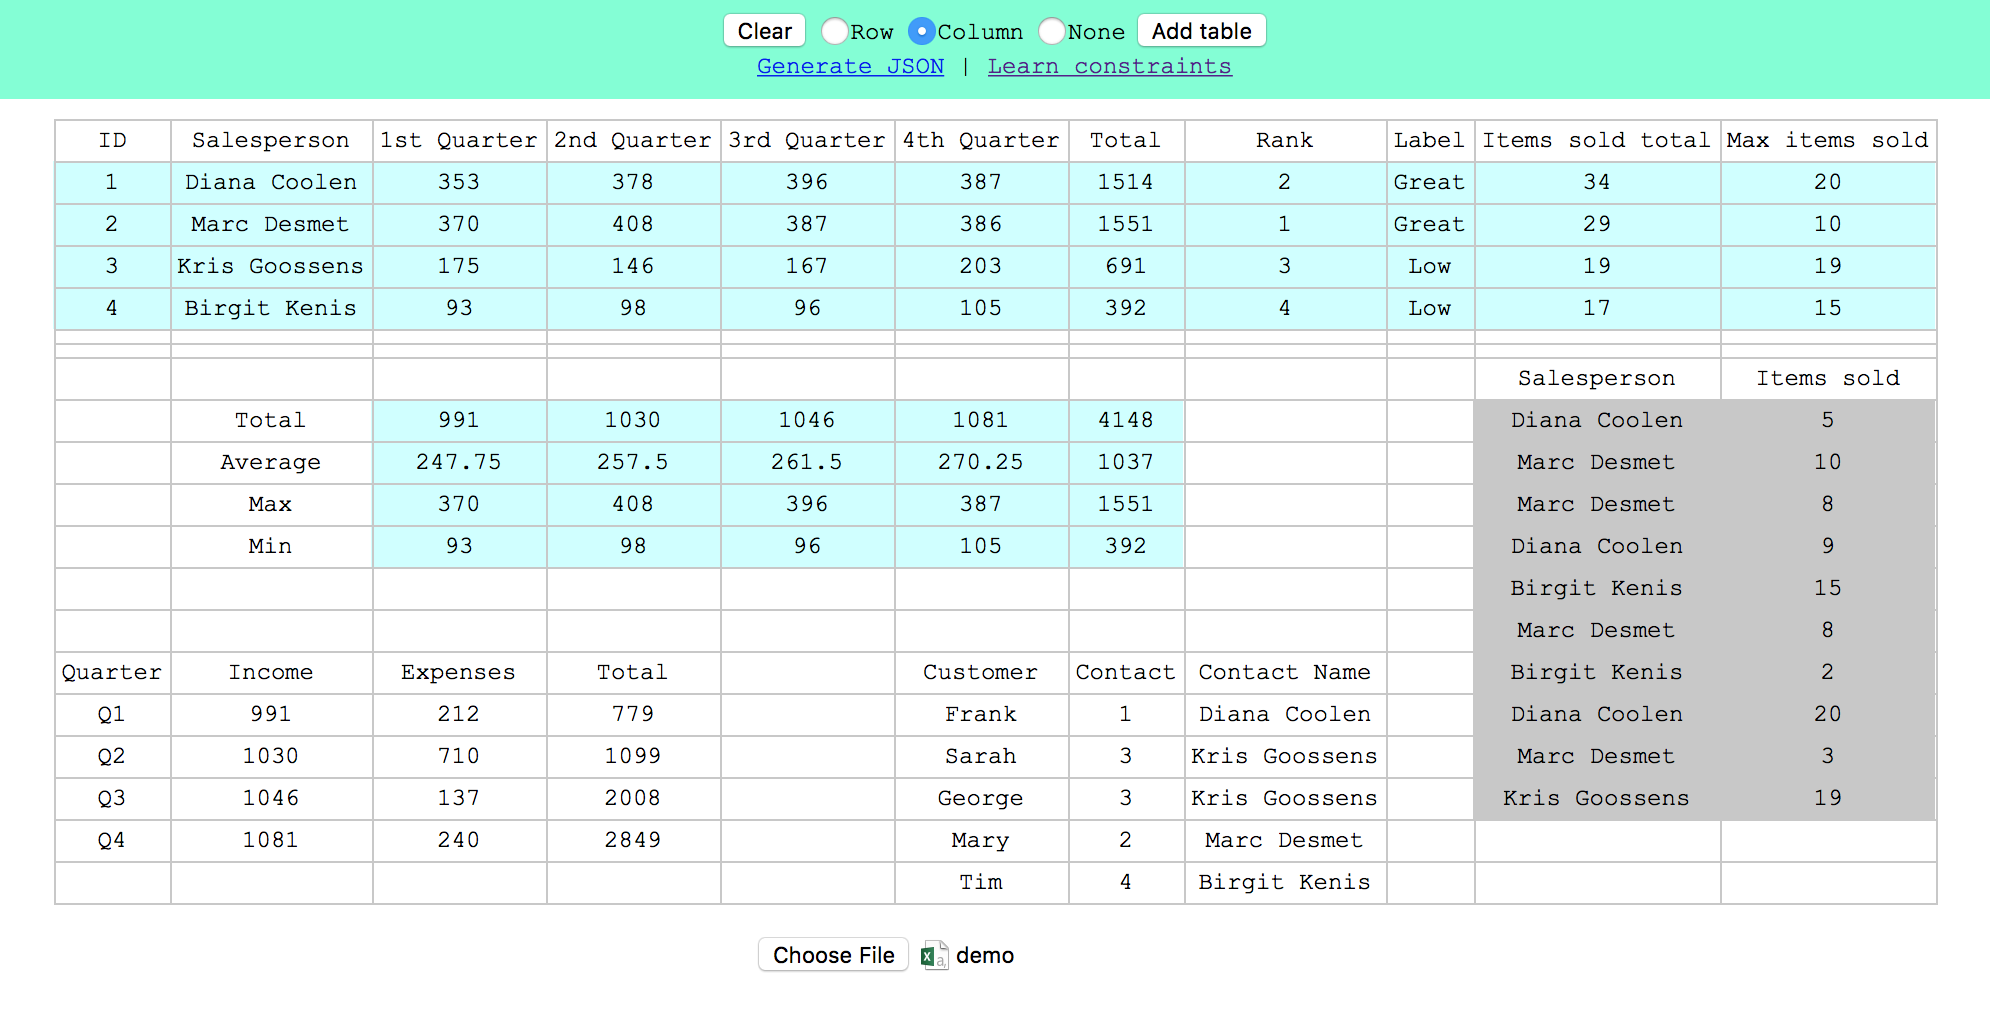
\includegraphics[width=1\linewidth]{figures/tabletool.png}
%   \caption{This simple table selection tool allows users to select rectangular ranges of cells corresponding to (headerless) tables.
%   An explicit orientation can also be provided.}
%   \label{fig:visual_tool}
% \end{figure}

Instead, we assume tables are specified by means of their coordinates within a spreadsheet and optionally a fixed orientation of each table. The orientation can be used to indicate that a table should be interpreted as having only rows or only columns.

We developed two simple prototypes to help with the specification of the tables:
%This information can be provided manually or generated automatically.


\paragraph{Automatic detection}
%As mentioned above, automatic detection of headers and tables is a complex task.
%Therefore, we define a restricted setting in which the task becomes easy enough to be automated.
Under the following two assumptions, the table detection task becomes easy enough to be automated; 1) tables are rectangular blocks of data not containing any empty cells; and 2) tables are separated by at least one empty cell from other tables.
The sheet is then processed row by row, splitting each row into ranges of non-empty cells and appending them to adjacent ranges in the previous row.
Headers can be detected, for example, by checking if the first row or column contains only textual values. If a header row (column) is detected, it is removed from the table and the orientation of the table is fixed to columns (rows), otherwise, we assume there is no header and the orientation is not fixed.

\paragraph{Visual}
The above assumptions do not hold for many tables. However, since the specification of tables is usually easy for humans, we propose a second approach which allows users to indicate tables using a visual tool (screenshots are available in the accompanying github repository with meta-data\footnote{\url{https://github.com/SergeyParamonov/TaCLe}\label{github-link}}).
Users select tables excluding the header and optionally specify an orientation.
The tool then generates the specification of the tables automatically.





\subsection{Block detection} \label{sec:make_groups}
%A spreadsheet may contain multiple tables, and a table in turn will contain multiple (type-consistent) blocks.
The goal of the block detection step is to partition tables into maximally type-consistent (all-numeric or all-textual) blocks.
%We generate blocks automatically, partitioning tables into maximal type-consistent blocks.
First, we preprocess the spreadsheet data so that currency values and percentual values are transformed into their corresponding numeric (i.e. integer or floating point) representation (e.g. $2.75 \$$ as $2.75$ or $85\%$ as~$0.85$).
Then, each table is partitioned into maximal type-consistent blocks.

To find row-blocks, each row is treated as a vector and must be type-consistent; similarly for columns and column-blocks. Then, adjacent vectors that are of the same type are merged to obtain the maximally type-consistent superblocks.


\subsection{Algorithm}
\label{sec:algo}
Our method assumes that constraint templates and maximal blocks are given and solves the \tcl~problem by checking for each template $s$: what combination of maximal blocks can satisfy the signature (\textit{superblock assignment}) and which specific \textit{subblock assignments} satisfy both the signature and the definition.
The pseudo-code of this approach is shown in Algorithm~\ref{algo:tcl}.
%For every constraint template~$s$, the algorithm first generates all combinations of superblocks (i.e. superblock assignments) that are consistent with the signature.
%In a second step it looks at every superblock assignment and finds subassignments that satisfy the signature and definition of~$s$.


This separation of checking the \textit{properties} of superblock assignments from checking the \textit{actual data} in the subblock assignment controls the exponential blow-up of combinations to test. Furthermore, we use constraint satisfaction technology in the first step to efficiently enumerate superblock assignments that are compatible with the signature. %These are the two key properties of our approach.

\newcommand{\temps}{\ensuremath{S}}
\begin{algorithm}[t]
  \begin{algorithmic}[1]
    \footnotesize
    \State \textbf{Input:} $\temps$ -- constraint templates, $\blocks$ -- maximal blocks
    \State \textbf{Output:} $C$ -- learned constraints

    \Procedure{LearnConstraints}{$\blocks$, $\temps$}
      \State $C \gets \emptyset$ %\Comment{The set of constraints}
      \ForAll{$s~\mathbf{in}~\temps$} \label{algo:tcl:for}
        %\State $n \gets$ number of arguments of template $s$
        \State $A \gets \generategroups(s, \blocks)$  \label{algo:tcl:super}
        \ForAll{$(\sbl{1}, \dots, \sbl{n}) \in A$}
        \State{$A' \gets \findassignment(s, (\sbl{1},\dots,\sbl{n}))$}
        \ForAll{$(\sbl{1}',\dots,\sbl{n}') \in A'$}
            \State $C \gets C \cup \{ c_s(\sbl{1}', \dots, \sbl{n}') \}$
          \EndFor
        \EndFor
      \EndFor
      \State \Return $C$
    \EndProcedure
\end{algorithmic}
\caption{Learn tabular constraints}
\label{algo:tcl}
\end{algorithm}





\subsubsection{Generating superblock assignments (Step 3a)}
\label{sec:algo:super}
\
% Let there be $b$ blocks and let~$s$ have~$n$ arguments, then a simple generate-and-test method would have to test $b^n$ combinations (given that blocks can be repeated), which can grow very rapidly with $b$, depending on $n$.

Given a constraint template~$s$ and the set of all (maximal) superblocks~\blocks, the goal is to find all combinations of superblocks that are compatible with the constraint signature.
An argument assignment $(\sbl{1}, ... \sbl{n})$ is \textit{compatible} with the signature of template $s$ if for each block $\sbl{i}$ there exists at least one subblock $\sbl{i}' \sqsubseteq \sbl{i}$ that satisfies the signature.

The choice of one argument can influence the possible candidate blocks for the other arguments, for example, if they must have the same length.
Instead of writing specialized code to generate and test the superblock assignments, we make use of the built-in reasoning mechanisms of constraint satisfaction solvers.

A Constraint Satisfaction Problem (CSP) is a triple $(V,D,C)$ where $V$ is a set of \textit{variables}, $D$ the domain of possible values each variable can take and $C$ the set of constraints over $V$ that must be satisfied.
In our case, we define one variable $V_i$ for each argument of a constraint template.
Each variable can be assigned each of the maximal blocks in \blocks, so the domain of the variables consists of $|\{\blocks\}|$ block identifiers.

%Finding candidate groups for a \template~$t$ can be seen as a Constraint Satisfaction Problem (CSP) dependent on the \CSignature of~$t$.
%For every argument in~$t$ we consider all groups~\groups (or all candidates from a more general constraint) and prune these candidate groups using their types and other requirements imposed by the templates \CSignature, such that a group~$G \in \groups$ is selected if there is at least one subgroup~$G' \subseteq G$ that satisfies the \CSignature.

To reason over the blocks, we add to the constraint program a set of background facts that contain the properties of each block, namely its type, table, orientation, size, length and number of rows and columns.

\begin{table}[tbh]
  \caption{Translation of signature requirements to superblock constraints. The following need not be relaxed: $\plength(B) = x$, $\por(B) = x$, $\ptable(B) = x$ and $\psize(B) \geq x$.}
  \label{tbl:translation}
  \begin{tabularx}{\linewidth}{lX}
    \textbf{Requirement} & \textbf{Superblock constraint} \\ \hline \hline
    $\ptype(B) = x$ & $\mathit{basetype}(\ptype(B)) = \mathit{basetype}(x)$ \\ \hline
    $\psize(B) = x$ & $\psize(B) \geq x$ \\ \hline
    $\pcols(B) = x$ & $\mathit{if}~\por(B) = \mathit{column}: \pcols(B) \geq x$ \\ 
    & $\mathit{if}~\por(B) = \mathit{row}: \pcols(B) = x$ \\ \hline
    $\prows(B) = x$ & $\mathit{if}~\por(B) = \mathit{column}: \prows(B) = x$ \\ 
    & $\mathit{if}~\por(B) = \mathit{row}: \prows(B) \geq x$
  \end{tabularx}
\end{table}

The actual constraints must enforce that a superblock assignment is \textit{compatible} with the requirements defined in the signature.

Table~\ref{tbl:translation} shows how the conversion from requirements of the signature to CSP constraints works:
Requirements on the lengths, orientations and tables of blocks can be directly enforced since they are invariant under block containment~($\sqsubseteq$).
Typing requirements need to be relaxed to check only for base types (numeric and textual).
Minimum sizes can be directly enforced, but exact size requirements are relaxed to minimum sizes, since blocks with too many vectors contain subblocks of the required (smaller) size.
Finally, restrictions on the number of rows or columns behave as length or size constraints based on the orientation of the block they are applied to.
Subgroups of row-oriented (column-oriented) blocks will always have the same number of columns (rows), however, the number of rows (columns) might decrease.

The $\generategroups(\textit{s,\blocks})$ method will use these conversion rules to construct a CSP and query a solver for all solutions.
These solutions correspond to the valid superblock assignments for constraint template~$s$.

\begin{example}
%Br and Bx are numeric; rows(Bx) ⇤ 2; and columns(Bx ) = length(Br )

  Consider the constraint template $\ecsumr{\sbl{r}}{\bsbl{x}}$, then the generated CSP will contain two variables $V_r, V_x$ corresponding to arguments~$\sbl{r}$ and~$\bsbl{x}$.
  Given maximal blocks~\blocks, the domain of these variables are $D(V_r) = D(V_x) = \{ 1, \dots, |\blocks| \}$.
  Finally, the signature of $\ecsumr{\sbl{r}}{\bsbl{x}}$ (see Table~\ref{table:constraints}) will be translated into constraints:
  \begin{align*}
    & \numeric(V_r) \land \numeric(V_x) \land \pcols(V_x) \geq 2 \\
    & (\por(V_x) = \mathit{column}) \Rightarrow (\prows(V_x) \geq \plength(V_r)) \\
    & (\por(V_x) = \mathit{row}) \Rightarrow (\prows(V_x) = \plength(V_r))
  \end{align*}
  %Every solution is a tuple of values for~$V_r$ and~$V_x$ corresponding directly with a superblock assignment over~\blocks.
\end{example}





\subsubsection{Generating subblock assignments (Step 3b)}
\label{sec:algo:subgr}

Given a superblock assignment $(\sbl{1}, \dots, \sbl{n})$ from the previous step, the goal is to discover valid \textit{subassignments}, i.e. assignments of subblocks $(\ssbl{1}, \dots, \ssbl{n})$ (for all $i$, $\ssbl{i} \sqsubseteq \sbl{i}$) that satisfy both the signature and the definition of template~$s$.

%While the previous step reasoned about the \textit{properties} of blocks, in this step we will also reason about the actual \textit{content} of the blocks, that is, the data.
\begin{example}
  Consider the sum-over-rows constraint template $\ecsumr{\sbl{r}}{\bsbl{x}}$.
  An example superblock assignment from Figure~\ref{fig:main_example} is $(\sbl{r}, \bsbl{x}) = (\range{T_1}{\rangeall}{\rangeto{3}{8}}, \range{T_1}{\rangeall}{\rangeto{3}{8}})$.
  Note that this assignment does not satisfy the signature yet because $\sbl{r}$ contains more than one vector.
  This step aims to generate subassignments $(\sbl{r}' \sqsubseteq \sbl{r}, \mathbf{\sbl{x}}' \sqsubseteq \mathbf{\sbl{x}})$ that do satisfy the signature and test whether they satisfy the definition:
  $\forall i, \sbl{r}[i] = \sum_{j = 1}^{length(\bsbl{x})} \mathit{row}(i, \bsbl{x})[j]$.
  In Figure~\ref{fig:main_example} there is exactly one such subassignment: $(\range{T_1}{\rangeall}{7}, \range{T_1}{\rangeall}{\rangeto{3}{6}})$.
\end{example}

In this step, we could also formulate the problem as a CSP. %However, the search space is much smaller, e.g. $O(nm^2)$ with $n$ the number of arguments of the template and $m$ the size of the largest block.
However, few CSP solvers support floating point numbers, which are prevalent in spreadsheets.
Furthermore, in a CSP approach we would have to \textit{ground} out the definition for each of the corresponding elements in the vectors.
This is inefficient, as already such blocks may not satisfy the signature or the first elements in the data may not satisfy the definition.

\begin{algorithm}[tbh]
  \begin{algorithmic}
    \footnotesize
    \Procedure{Subassignments}{$s$, $(\sbl{1}, \dots, \sbl{n})$}
    \State $n \gets$ number of arguments of template $s$
    \State $A_{sub} \gets \emptyset$
    \ForAll{$(\sbl{1}', \dots, \sbl{n}') \textbf{ where } \forall i: \sbl{i}' \sqsubseteq \sbl{i}  \land \textit{disjoint}_{j \neq i}(\sbl{i}', \sbl{j}')$}
      \If{$\textit{Sig}_s(\sbl{1}',\dots,\sbl{n}') \land \textit{Def}_s(\sbl{1}',\dots,\sbl{n}')$}
        \State $A_{sub} \gets A_{sub} \cup \{ (\sbl{1}', \dots, \sbl{n}') \}$
      \EndIf
    \EndFor
\Return $A_{sub}$
\EndProcedure
\end{algorithmic}
\caption{Generate-and-test for $\findassignment$}
\label{algo:gen-test-subblocks}
\end{algorithm}


On the other hand, a simple generate-and-test approach, as illustrated in Algorithm~\ref{algo:gen-test-subblocks}, will usually suffice.
%However, the actual implementation is specified for every constraint template separately, allowing different methods to be used based on the type of template.
%For this reason, the \sname system uses generate-and-test to implement $\findassignment$ for most constraint templates.
Given a superblock assignment, all disjoint subassignments are generated taking into account the required size, columns or rows.
For every (disjoint) subassignment the exact signature (e.g. subtypes will not have been checked yet) and definition will be tested and all satisfying subassignments are returned.



% \begin{verbatim}
% VERY PSEUDOcode:
% something recursive that handles vectors/
% subgroups differently like this?
% check(Groups, X, Test):
%   if |Groups| == 0:
%     forall i in ?: vector elements...
%       if not Test(X):
%         return []
%     return X
%   // else
%   all = []
%   Group = Groups.pop(0)
%   if vector(Group):
%     forall Vec in Group:
%       all += check(Groups, X + Vec, Test)
%   else:
%     forall Subgroup in Group:
%       all += check(Groups, X + Subgroup, Test)
%   return all
% \end{verbatim}

 %$G_1 = +(G_2, G_3) \leftrightarrow G_1 = +(G_3, G_2)$. \samuel{\tias{How are they stopped in the code? should be part of the pseud-code because not part of $Test(X)$?} will make it part of pseudo-code}

% \paragraph{Example 2, not used (should be replaced by pseudo-code above?)}
% Sum Product

% Implementation: finds subgroups based on assignments\\
% Method $Test(G_R, G_{O_1}, G_{O_2})$\\
% $If \lnot G_{O_1} < G_{O_2}: Reject~\#~Canonicity$\tias{ill-defined, $G_{O_1}$ is a group and $<$ not defined on it (on vector identifiers rather than content?)}\\
% $If data(G_R) = data(G_{O_1}) \bullet data(G_{O_2}): Accept$ \tias{does not show that reasons over content of vectors}
% \\\\
% Method $FindSubgroups(Assignments)$\\
% $Return \{ (G_R', G_{O_1}', G_{O_2}') | \exists (G_R, G_{O_1}, G_{O_2}) \in Assignments \land G_R' \subseteq G_R \land G_{O_1}' \subseteq G_{O_1} \land G_{O_2}' \subseteq G_{O_2} \land Test(G_R', G_{O_1}', G_{O_2}') \}$ \tias{does not enforce size of subgroups (e.g. vectors)?}





\subsection{Optimizations} \label{sec:opts}
This section discusses various design decisions and optimizations aimed at improving the speed, the extensibility of our system and the elimination of redundant constraints.

\subsubsection{Template dependencies}
As discussed in Section~\ref{sec:form:dependencies}, some constraint templates depend on others by including templates they depend on in their signature (see Table~\ref{table:constraints}).

In Inductive Logic Programming, one often exploits implications between constraints to structure the search space~\cite{luc_book}.
Our approach uses the dependencies between templates to define a dependency graph.
We assume that signatures do not contain equivalences or loops, and hence the resulting graph is a directed acyclic graph (DAG).
Figure~\ref{fig:learning_order} shows the dependency graph extracted from the signatures in Table~\ref{table:constraints}. 
Constraint templates that have no dependencies are omitted.

\begin{figure}[t]
  \centering
  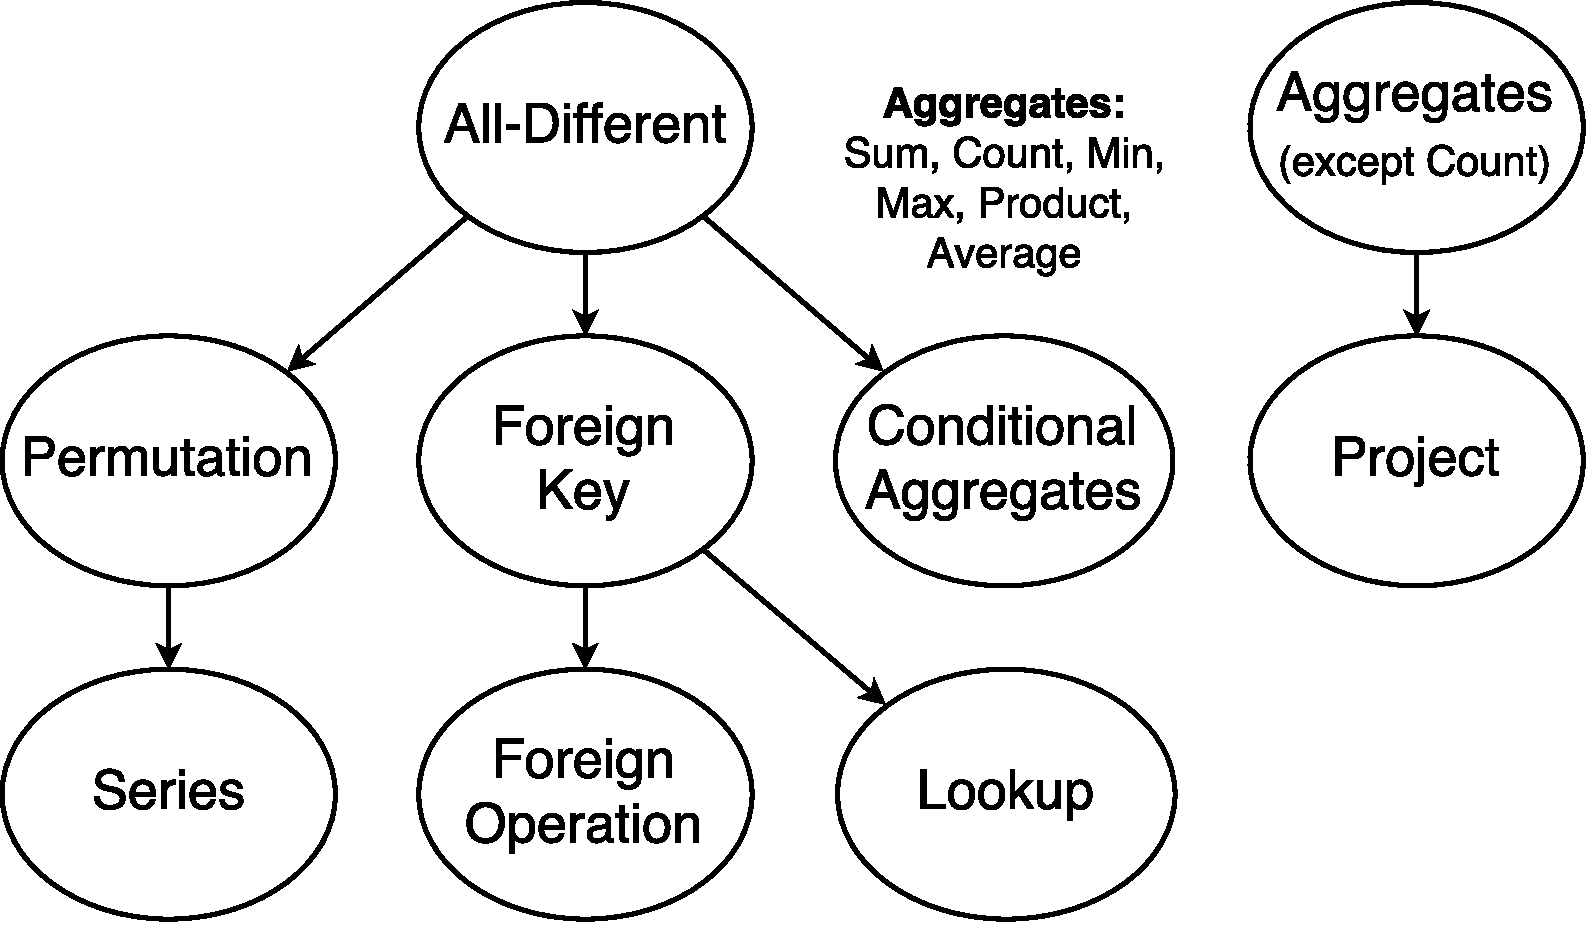
\includegraphics[width=0.50\linewidth]{figures/constraint_dependency2.pdf}
  \caption{Dependency graph of Table~\ref{table:constraints}; an arrow from~$s_1$ to~$s_2$ indicates that $s_2$ depends on~$s_1$ (its signature includes $s_1$).
  }
  \label{fig:learning_order}
\end{figure}

Using the dependency graph~(\dependencies) we can reorder the templates such that a template occurs after any template it depends on.
Concretely, in Algorithm~\ref{algo:tcl} line \ref{algo:tcl:for} the input templates~$\temps$ are handled following an ordering that agrees with the partial ordering imposed by~\dependencies (e.g. \textit{ALLDIFFERENT} before \textit{FOREIGNKEY}).
When using this ordering, templates later in the ordering can use the learned constraints of the templates they depend on.
To enable this reuse of constraints, the set of learned constraints $C$ is added to the argument of \generategroups on line \ref{algo:tcl:super}.

The previously learned constraints are used to speed up the \generategroups step. For constraint templates where some arguments are also part of a constraint that it depends on, it is not needed to search for superblocks and subblocks from scratch. Instead, one can start from all and only the actual argument assignments of the base constraint, and only search matching superblocks for the remaining arguments.

\begin{example}
  Consider $\ecfkey{\sbl{fk}}{\sbl{pk}}$, which states that every value in $\sbl{fk}$ also exists in $\sbl{pk}$; its signature includes $\ecalldiff{\sbl{pk}}$. There are 18 \textit{ALLDIFFERENT} constraints to be found in Figure~\ref{fig:main_example}, hence, the \generategroups only needs to check which superblocks for $\sbl{fk}$ are compatible (different table, same type) with these 18 assignments to $\sbl{pk}$.
\end{example}

Instead of generating one CSP to find all assignments, a CSP is generated for every known assignment of the depending constraint (and variables involved), which then searches for all assignments completing this partial assignment.
The procedure to generate CSPs remains the same otherwise.





%\subsubsection{Constraint solvers}
%\samuel{Tias, Sergey, have a look at his section, I'm torn about rewriting it, feeling it should either be reduced or expanded, especially the second part.}
%Generic constraint solving technology can be used for the candidate group generation as well as for enumerating the satisfying subgroups.
%Constraint solvers can be categorized as being stand-alone solvers, meaning that they have a text-based modeling language in which the CSP must be formulated, and \textit{embedded}, meaning that they have a programmatic API to formulate the CSP.
%
%\sname supports the ASP \cite{whaisasp} formalism, using the stand-alone Clingo 4.5.4 \cite{clingo} solver, the MiniZinc language \cite{minizinc} with the stand-alone Gecode 4.4.0 solver (which supports floats) and uses an embedded Python-based CP solver \cite{python_constraint}.
%The constraint signature that must be satisfied to generate the groups can be specified in each of the tree formalisms, to ease prototyping and extendability towards new constraints. The embedded solver is fastest as it does not have the overhead of file-writing and calling an external program, and is used in the experiments below.





\subsubsection{Redundancy}
We consider two types of redundancy that we aim to eliminate during search.
As noted in Section~\ref{sec:form:dependencies}, for some constraint templates there are \textit{symmetries} over the arguments that lead to trivially equivalent solutions, for example, $\ecprod{\sbl{R}'}{\sbl{1}'}{\sbl{2}'} \Leftrightarrow \ecprod{\sbl{R}'}{\sbl{2}'}{\sbl{1}'}$.
Such duplicates are avoided by defining a \textit{canonical} form for these constraints.
In practice, we define an arbitrary but fixed block ordering and require those blocks that are interchangeable to adhere to this ordering.
Moreover, among the semantically equivalent constraints product (\ecprod{\sbl{R}'}{\sbl{1}'}{\sbl{2}'}) and division (\eccalc{\sbl{1}'}{\sbl{R}' / \sbl{2}'}) we only added product, as well as only difference (\ecdiff{\sbl{r}}{\sbl{1}}{\sbl{2}}) and not sum (\eccalc{\sbl{1}}{\sbl{r} + \sbl{2}}). However, division and sum could easily be added, as they could be added explicitly in post-processing based on the matching product and difference constraints.


A last type of redundancy we chose to reduce is that there may be multiple \textit{overlapping} subblocks that satisfy the definition of a constraint template.
For example, consider the constraint $\ecsumc{\sbl{r}}{\range{T}{\rangeall}{\rangeto{1}{n}}}$ where $\range{T}{\rangeall}{\rangeto{k}{n}}$ consists of only zeros, then $\ecsumc{\sbl{r}}{\range{T}{\rangeall}{\rangeto{1}{j}}}$ will be true for all $k - 1 \leq j \leq n$.
In \sname we have, therefore, chosen to only consider \textit{maximal} subblocks.

In some cases a maximal subblock might falsely include irrelevant columns.
Consider superblock $\bsbl{x} = \range{T}{\rangeall}{\rangeto{1}{3}} = [[200, 300], [200, 150], [1, 2]]$ and $\sbl{r} = [200, 300]$, then \sname will find the constraint $\eccalc{\sbl{r}}{\textit{MAX}(\range{T}{\rangeall}{\rangeto{1}{3}})}$.
Should the target constraint be $\eccalc{\sbl{r}}{\textit{MAX}(\range{T}{\rangeall}{\rangeto{1}{2}})}$, then $\range{T}{\rangeall}{3}$ must be split off into a separate block.

Alternatively, we can output all valid assignments instead of only maximal subblocks, e.g. $\eccalc{\sbl{r}}{\textit{MAX}(\range{T}{\rangeall}{1})}$, $\eccalc{\sbl{r}}{\textit{MAX}(\range{T}{\rangeall}{\rangeto{1}{2}})}$ and $\eccalc{\sbl{r}}{\textit{MAX}(\range{T}{\rangeall}{\rangeto{1}{3}})}$, however, this might produce many redundant constraints including constraints that accidentally cover too little data.





\subsubsection{Constraints} \label{sec:which_cons}
The \samuel{count} constraints that are currently supported in our system are shown in Table~\ref{table:constraints}.
We included most formulas that we encountered in tutorial spreadsheets including the popular \textit{SUM} and \textit{LOOKUP} constraints\footnote{\href{https://support.office.com/en-us/article/Excel-functions-by-category-5F91F4E9-7B42-46D2-9BD1-63F26A86C0EB}{https://support.office.com/en-us/article/Excel-functions-by-category-5F91F4E9-7B42-46D2-9BD1-63F26A86C0EB}}.
We also added three structural constraints (\textit{ALLDIFFERENT}, \textit{PERMUTATION} and \textit{FOREIGNKEY}) so that they can be used in the signature of other constraint templates; they are also popular in constraint satisfaction~\cite{modelseeker}.

For \textit{FOREIGNKEY}, \textit{LOOKUP}, aggregates and \textit{PROJECT} we use custom, optimized methods to find subassignments.
Instead of the more generic generate-and-test implementation, we use, for example, caching, maximal range-finding and partial tests.
While conditional aggregates use generate-and-test, they employ similar optimizations in their test method.

Based on the assumptions that most subassignments will not satisfy a constraint template, the implementations are geared to \textit{fail-fast} when possible.
Specifically, the tests try to prove that a subassignment does not satisfy a constraint template as fast as possible.
For example, it can be often shown that a constraint does not hold by only looking first entries of every subblock (e.g. if $\sbl{r}[0] \neq \sbl{1}[0] \times \sbl{2}[0]$ then $\sbl{r} = \sbl{1} \times \sbl{2}$ does not hold).
As a result, the time to check if a subassignment satisfies a constraint templates with a fail-fast implementation requires constant time\footnote{If the number of entries to look at is bounded by a constant, the vector lengths are smaller than the number of subassignments to test ($a$) and the time to test subassignments that satisfy the constraint is $O(a)$, then the time to test a subassignment is amortized $O(1)$} in most cases and does not depend on the length of the vectors.


%\paragraph{Theoretical analysis of runtime, this does not belong in experiments}\tias{move to technical section}\sam{Has to be moved yet to 'Constraints' section, explaining fail-fast}
%For most constraint templates the time required to check whether a subassignment satisfies the template is linear in the size of the subassignment (the number of subblocks and their size).
%For a constraint with arity~$n$, and a subassignment consisting of $n$~blocks with $m$~vectors of length~$k$, the worst case complexity becomes $O(n * m * k)$.
%However, in practice, most subassignments will not satisfy the constraint template.
%Since our implementation tries to account for this by failing fast\tias{explain more precisely what you mean with 'failing fast'}, the amortized time is constant in the length of the vectors~$k$, unless $k$~is very large\footnote{Specifically, if $k$ is much larger than the number of candidate subassignments} or many constraints hold in the data.
%For templates requiring their arguments to be single vectors $m$~is~$1$, and the total complexity for checking a subassignment becomes~$O(n) \simeq O(1)$ (since $n$ is typically small).



%Their dependencies are reflected in their \CSignature and shown in Figure~\ref{fig:learning_order}.
%These constraints have been selected based on the most-used Excel functions as well as their occurrence in various example spreadsheets we observed.

%Note that \samuel{Motivate why product, not sum (=diff) you only need one, hardcoded preference for display - diff not present - pruning relation?}

% Extending the system with a new constraint template amounts to \tias{TODO: samuel, explain how to define syntax; signature-for-groupgen; signature-for-def; definition}


% \begin{equation}
%   \forall i{:}~ v_r[i] \leq v[i] < v_r[i] + 0.5
%   \label{eq:floor_extension}
% \end{equation}


% \subsection{Workflow}
% \begin{algorithm}[thb]
%   \begin{algorithmic}
%     \footnotesize
%     \State \textbf{Input:} $D$ -- dataset, \constraints -- constraints, \dependencies -- dependencies \\(optional: tables $T$, groups $G$)
%     \State \textbf{Output:} $S$ -- learned constraints with their satisfaction assignment
%     \If{$T$ is \textbf{not} provided}
%       \State $T \gets \extracttables(D)$
%     \EndIf
%     \If{$G$ is \textbf{not} provided}
%       \State $G \gets \extractgroups(D, T)$
%     \EndIf
%     \State $S \gets \learnconstraints(G,\constraints,\dependencies)$
%     \State \Return $S$
% \end{algorithmic}
% \caption{Workflow}
% \label{algo:workflow}
% \end{algorithm}

% \textbf{Approach}
% \begin{itemize}
%   \item Notation
%   \item Algorithm (select constraints, find assignments, find solutions)
% \end{itemize}

% \samuel{Move next to subgroup satisfaction search}
% \section{Declarative modeling}

\newcommand{\runtotal}{16.12}
\newcommand{\runtotalstd}{0.62}

\newcommand{\runfile}{0.50}
\newcommand{\runfilestd}{0.02}

\newcommand{\benchsize}{??}

\section{Evaluation}\label{sec:evaluation}
In this section we experimentally validate our approach.
We first explain the experimental setup and illustrate it on the example in Figure~\ref{fig:main_example}, we then investigate the effectiveness of our method on generated spreadsheets, after which we evaluate our method on spreadsheets from various sources.

\paragraph{Experimental setup}
\label{sec:evalualtion:method}
All spreadsheets used in the experiments are in CSV format, and for each we have ran the table extraction tool once (using a combination of the rather primitive automatic detection + visual verification that the tables are meaningful (e.g. merge split-up tables because of None values, or remove headers of all-textual tables).
\samuel{Should we not say just with the visual tool?}
 \\ % split of weird sentence
Blocks are detected automatically using our block detection algorithm (Section~\ref{sec:make_groups}) unless a spreadsheet contains ambiguous \textit{None} values.
For those ambiguous cases the blocks are specified manually. \samuel{I have yet to make this more precise}

% Group definitions are only specified if the spreadsheet contains ambiguous \textit{None} values. \tias{What does this mean, 'group definitons'?? Is this 'block detection' (Sec 4.2), if so, how do we explain this process??} 

All spreadsheets also have a set of ground-truth of constraints, we call these the \textbf{intended} constraints, that are expected to be (re-)discovered.
These were determined by us using either the formulas of the original sheet (if present), or inferring them based on, for example, the header names in the sheet.
In the following experiments, we focus on spreadsheets specifically and hence only include \textit{functional} constraints, constraints that can be expressed as formulas. We ignoring structural constraints such as \textit{ALLDIFFERENT}, \textit{FOREIGNKEY} and \textit{PERMUTATION}. All constraints are stored in their canonical form. 5 spreadsheets contained rows or columns that were entirely identical, and any intended constraint involving one such vector was also added for the equivalent vectors. \samuel{They are usually not copied}

Section~\ref{sec:which_cons} discusses the 32 constraints currently supported by \sname \tias{It does, right? Should also contain '32' number}\sam{I will recount at the end}. Some of the intended constraints are currently outside of the scope of \sname however, more specifically nested mathematical or nested logical formulas. We denote by \textbf{supported} constraints the subset of intended constraints that the system can find in theory.

We will use recall and precision to measure how well our tool is performing. Recall is the fraction of intended constraints actually discovered by the system: $\frac{\text{intended discovered}}{\text{all intended}}$, while precision is the fraction of constraints found by the system that are indeed intended: $\frac{\text{intended discovered}}{\text{all discovered}}$.

All experiments were run using Python 3.5.1 on a Macbook Pro, Intel Core i7 2.3~GHz with 16GB RAM.
The constraint solver that is used by the superblock assignment phase (Step 3a) is python-constraint\cite{python_constraint}.



\subsection{Results on the running example}
For the example presented in Figure~\ref{fig:main_example},
\sname takes a few seconds to find the constraints listed in Figure~\ref{fig:sol_example}.
These include 5 spurious $\textit{RANK}$ constraints, e.g. $\ecrank{\range{T_1}{\rangeall}{1}}{\range{T_1}{\rangeall}{5}}$, that are true by accident.
Moreover, there is 1 \textit{LOOKUP} constraint that was not intended in the original spreadsheet (looking up ID based on Salesperson) and which is symmetric to the intended one (Salesperson based on ID).

Hence, for this example we achieve a recall of 100\% (all intended constraints are discovered) and a precision of $12/18 = 67\%$. All intended constraints are supported. The recall is as good as we hoped, but the precision is rather low. This is mostly due to the spurious RANK constraints. We note that the tables are quite short, which increases the chance of a constraint like \textit{RANK} to be true by chance; we expect less spurious constraints on larger datasets.

We now investigate three main questions that influence the quality of the solutions found by a constraint learning method:
\begin{itemize}
\item Q1: it may fail to find intended constraints if it takes too much time to find them; what are the factors that influence the runtime of the method most?
\item Q2: it may fail to find intended constraints because it does not support such constraints; how does or method perform on real spreadsheets?
\item Q3: it may find non-intended constraints; how many and what type of non-intended constraints are found on real spreadsheets?
\end{itemize}
We first investigate Q1 on generated spreadsheets, and Q2 and Q3 on a collection of real spreadsheets.


\subsection{Effectiveness on generated data}

\begin{figure}[t]
  \centering
  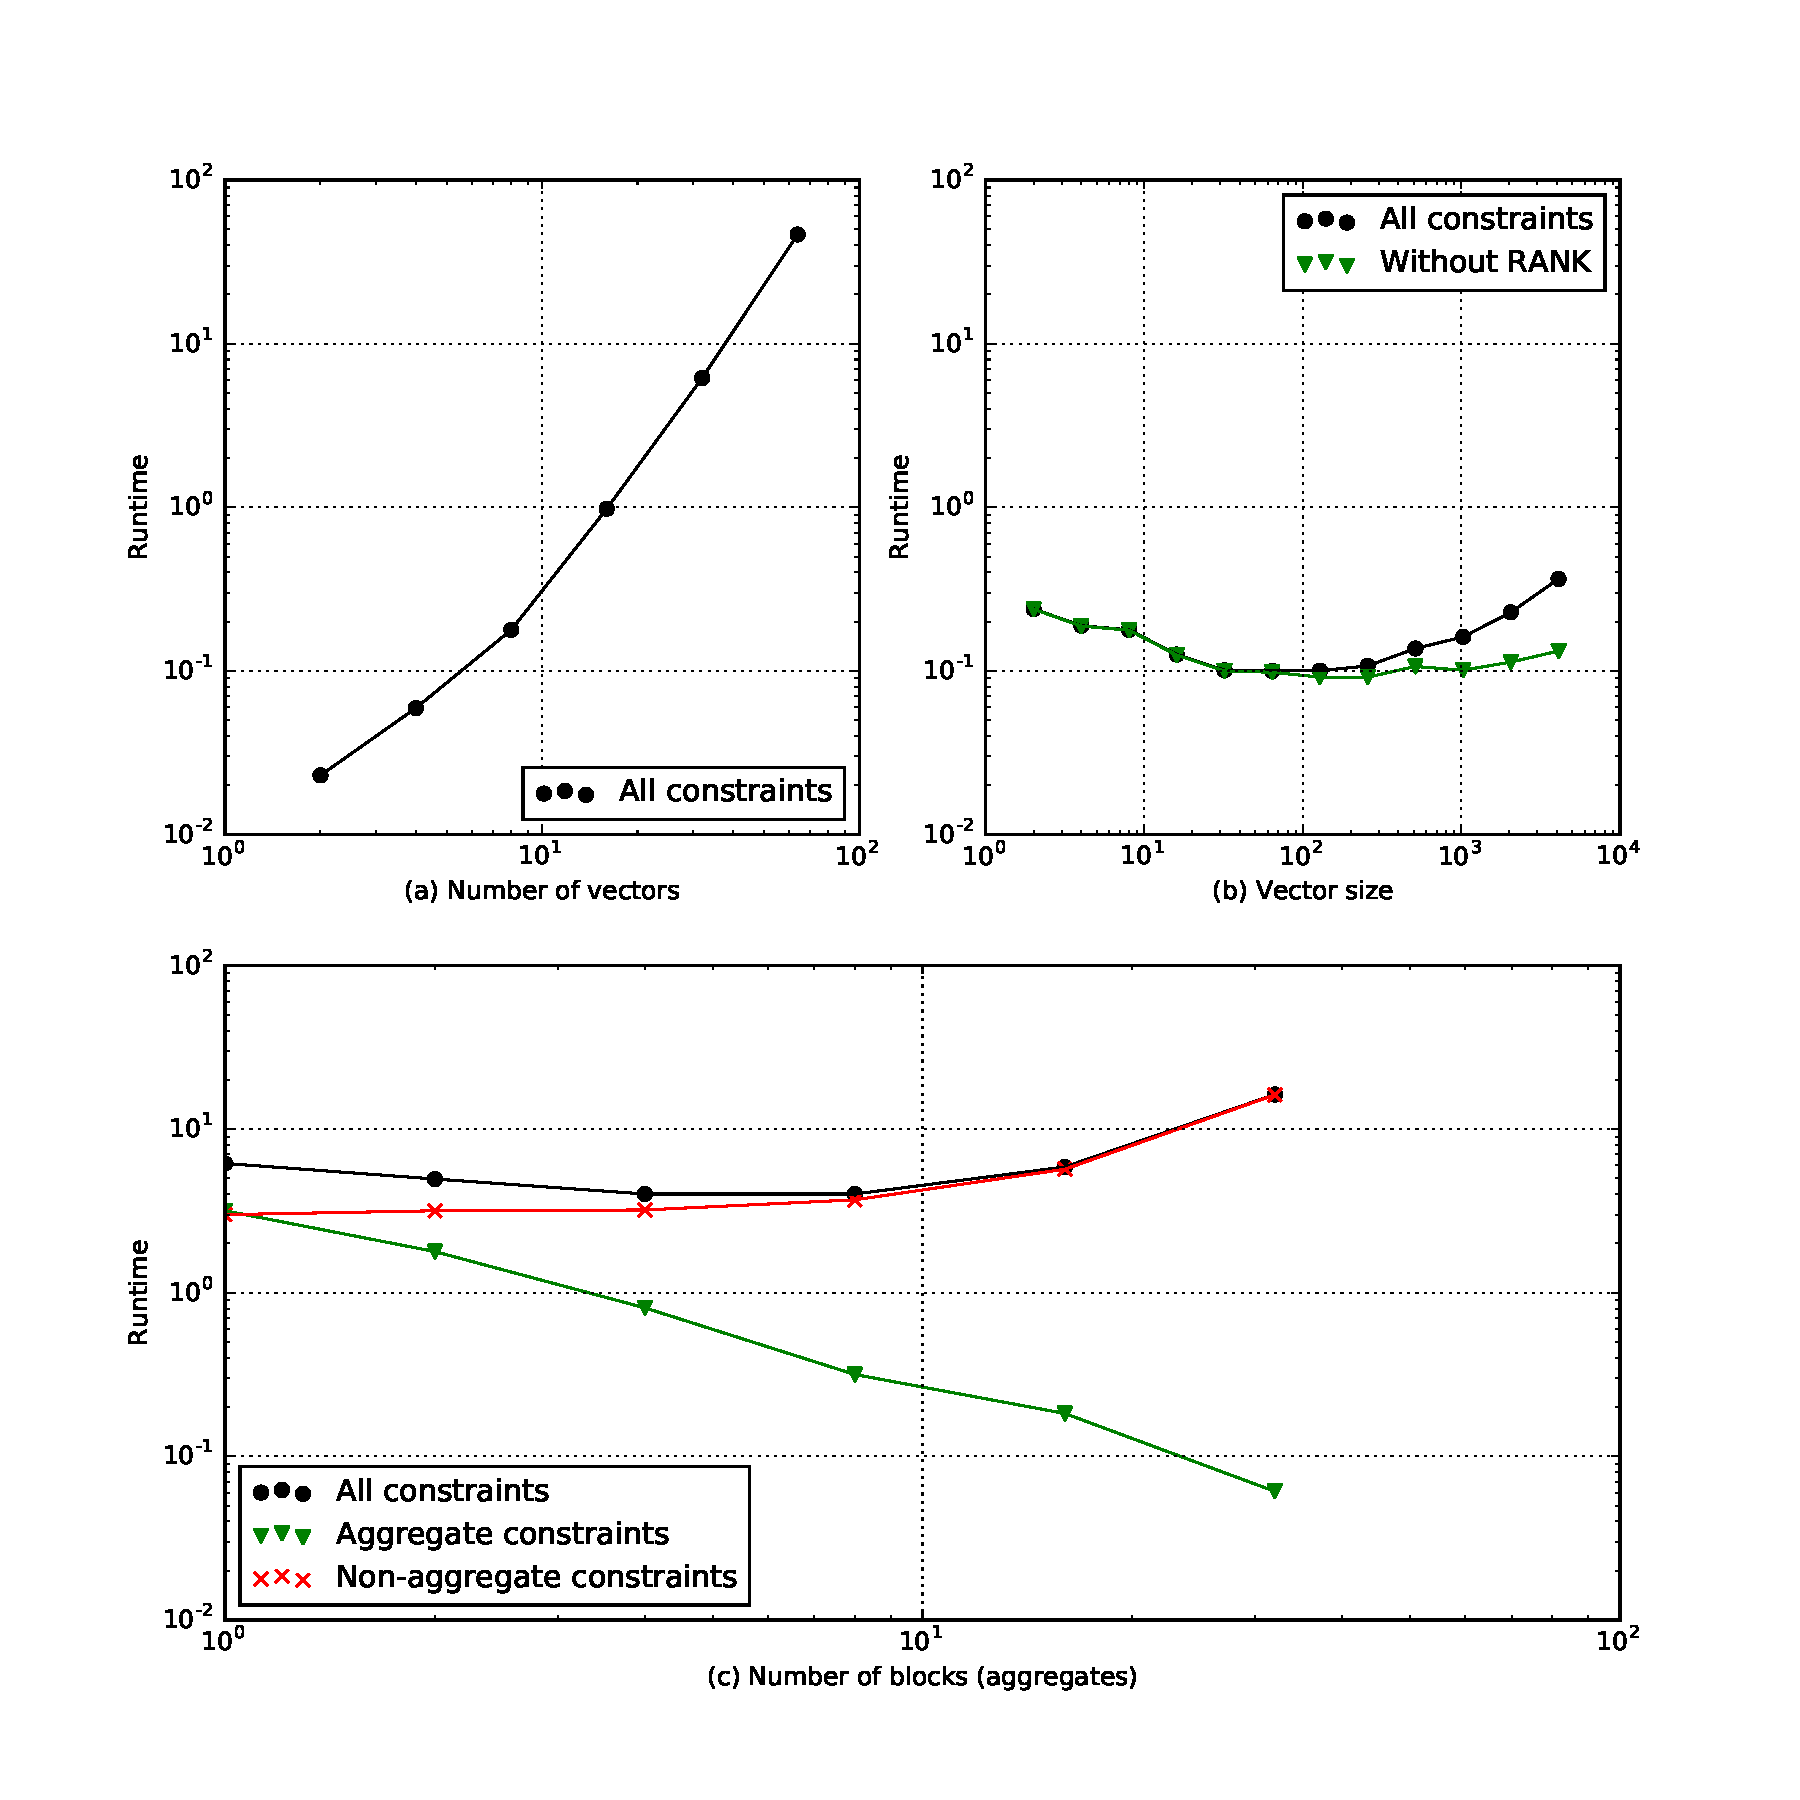
\includegraphics[width=1\linewidth]{figures/scatter_plots.pdf}
  \caption{Loglog plots of the experiments with synthetic (random) data. In plot~$a$ the number of vectors is increased; in plot~$b$ the size of the vectors is increased; and in plots~$c$ and~$d$ the number of blocks is increased.}
  \label{fig:runtime_analysis}
\end{figure}

In this section the impact on the running time is analyzed of 1)~the number of vectors; 2)~the length of the vectors; and 3)~the size of the blocks.
This analysis is accomplished by testing our system on generated spreadsheets.

Recall that our method uses a 2-phase approach where in the first phase, the superblock assignments are generated (Section~\ref{sec:algo:super} and in the second phase, the subblock assignments are generated (Section~\ref{sec:algo:subgr}).

\paragraph{Spreadsheet generation}
For our analysis, we perform multiple experiments on synthetically generated spreadsheets.

Many constraints require either numeric or discrete data, therefore, the type of cells also has an impact on the running time.
Since integers fulfill both of those typing restrictions, the generated spreadsheets contain only integer data.

One of the assumptions guiding the implementation is that most of the possible constraints are false.
To simulate this setting, the generated spreadsheets contain random data.
There will be few constraints that hold on these spreadsheets, however, random data is likely to produce vectors that fulfill the \textit{ALLDIFFERENT} constraint, which is a requirement for many other constraint templates.

In order to also analyse constraints that require their arguments to be picked from different tables, the spreadsheets are made up of two tables.
For one table the number of vectors and block size is fixed to two, while for the other table these properties are varied.
The number of vectors and the block size in the experiments are only reported for the adaptable table.
The length of the vectors can also be adapted and applies to both tables.
Unless otherwise mentioned, the adaptable table consists of one block containing all its vectors and by default the number of vectors and vector length are both~$8$.
%The running times for various configurations are plotted in Figure~\ref{fig:runtime_analysis}. % no such general pointer, specific pointers only

\paragraph{Effect of number of vectors}
Figure~\ref{fig:runtime_analysis}a shows the results of our experiments, in which \sname was run on generated spreadsheets containing an increasing number of (equally sized) vectors.
As shown in the figure, the number of vectors in a spreadsheet can have a significant impact on the running time.

This behavior is to be expected when not many superblock assignments can be discarded in phase~1, for example, when all vectors have the same type and size.
In this case, for a constraint template that requires $n$~single vector arguments and a spreadsheet with $v$~vectors, up to $\frac{v!}{(v - n)!}$ subassignments are generated throughout the algorithm.

Typically, we expect the number of generated subassignments to be much smaller in real world spreadsheets and, therefore, the running time to be less sensitive to the number of vectors.
This is because in phase~1 entire blocks can be disqualified that do not match the signature requirements, e.g. blocks of vectors with different lengths for the product constraint.
% \tias{Better move to 4.3.2? or have there too anyway, no new facts in 'experiment' section}\samuel{?}
\samuel{=> benchmark}


% Many constraints take single vector arguments, therefore, the total number of subassignments that are generated in the second phase of the algorithm depends on the number of vectors in the spreadsheet and the arity of the constraint.

% \tias{unclear, this is about phase 2, the number to test, or the actual testing of each? explain and relate to Sec 4.3.2 what aspect you are discussing here} to be tested depends on the number of vectors in the spreadsheets and the arity of the constraint.

% For a constraint template with arity~$n$ and $v$~vectors there are $n^v$ subassignments (or $\frac{n!}{(n - v)!}$ if the arguments have to be different). \tias{Better move to 4.3.2? or have there too anyway, no new facts in 'experiment' section}
% As the number of vectors in a spreadsheet increases, the running time will quickly be dominated by constraints with a larger arity.
% This effect is noticeable in our synthetic experiments when the number of (equally sized) vectors \tias{more details about equal sized: is this a strict requirement for this to happen? I assume this is worst case and does not happen that much in practice? (the next sentences half hint at that, be more explicit)} is increased (Figure~\ref{fig:runtime_analysis}a).

\paragraph{Effect of length of vectors}
%The benchmark experiments show that the number of cells in a spreadsheet has a very limited impact on the running time.
To measure the effect that the length of the vectors has on the running time, we ran our system on spreadsheets in which the length of the vectors was gradually increased.
Figure~\ref{fig:runtime_analysis}b summarizes our results and shows that the length of the vectors has a small impact on the performance for most templates.

As discussed in \samuel{???}, our implementation attempts to detect as fast as possible if a subassignments does not satisfy a constraint template.
Our experiments satisfy the assumption that the large majority of possible subassignments do not satisfy most constraints.
Therefore, the results confirm that our implementation is able to severely limit the impact of the length of vectors.

Most of the increase in running time can be attributed to the \textit{RANK} constraint.
The implementation is not always able to detect subassignments that do not satisfy \textit{RANK} quickly and often has to fall back to analyzing an entire vector.

\paragraph{Effect of block size}
To measure the effect of changing the block size, the number of vectors is set to~$32$ and the vectors are split into varying number of blocks (up to ~$32$).
Figure~\ref{fig:runtime_analysis}c shows the running times of \sname for various settings.
As the blocks become smaller, the total running time first decreases before increasing again.
Looking at the running times for aggregate constraints and non-aggregate constraints  separately reveals that they are affected differently by the block size.
For aggregate constraints (\samuel{xxx line}) the running time decreases with the block size, while for non-aggregate constraints (\samuel{yyy line}) the running time first stays more or less constant but then increases more strongly as the size of the blocks becomes very small.

Aggregate constraints, e.g. sum or max, have an argument that takes subblocks of varying sizes.
Contrary to non aggregate constraints, which only have single vector argument, superblock assignments from phase~1 are not split into single vectors subassignments in phase~2.
Instead, for an argument with variable size, the system tries to find any subblock of the given superblock that satisfies the constraint.
Since, for a superblock of size~$m$, the number of subblocks is $O(m^2)$ \samuel{ref?}, the search for aggregate constraints will be faster if there are more but smaller blocks\footnote{Consider, for example, $v$~vectors distributed over $b$~blocks of size $v/b$, the number of subblock candidates then is $O(b * v^2 / b^2) = O(v^2 / b)$}.

Non-aggregate constraints have only single vector arguments.
Therefore, the total number of subassignments generated by the algorithm is not influenced by the block size.
By splitting a set of vectors into many blocks, however, there will be a larger number of superblocks in phase~1 and, therefore, a larger number of superblock assignments have to be generated.
Recall that in phase~1 the algorithm additionally tests block level properties for every superblock assignment.
In the generated spreadsheets these tests can only disqualify few or no superblock assignments, therefore, it will be faster to group the same vectors into larger super blocks, generate fewer superblock assignments to test and split these into single vector subassignments in phase~2.

Splitting unrelated vectors into smaller subblocks can decrease the running time for some spreadsheets by reducing the workload for aggregate constraints.
However, the two phase approach is also well suited to operate on large blocks and eliminate superblock assignments that are not compatible with constraint template signatures. \samuel{Does this conclusion sound sound?}

% \tias{Point to figure to support this (actually, move that line into 4c??); also, if this is true, you are basically saying that the CP-based first phase is worse then the second phase? That kind-of demotivates the idea of using CP in first phase... What do you really want to share with the reader?}



\subsection{Effectiveness on real spreadsheets}
In order to test our approach on real data we assembled a benchmark of spreadsheets from three sources:
1)~spreadsheets from an exercise session for teaching Excel based on~\cite{excel_book}; 2)~spreadsheets from tutorials online; and 3)~publicly available \textit{data} spreadsheets such as real-world crime statistics or financial reports (available at the same repository\footref{github-link}).

Table~\ref{tbl:category_overview} gives an overview of the spreadsheets in the different categories and summarizes the results of our experiments.
% Notice that for the data category the average number of cells is higher while the number of intended constraints and tables is lower compared to the other categories. \tias{Weird here because purpose unclear, point to this when discussing some result for which this is important}

{\setlength{\tabcolsep}{0.33em}
\begin{table}[]
  \centering
  \caption{Summary of properties and results per spreadsheet category}
  \label{tbl:category_overview}
  \begin{tabular}{lccccccc}
 & \multicolumn{2}{c}{\textbf{Exercises} (9)} & \multicolumn{2}{c}{\textbf{Tutorials} (21)} & \multicolumn{2}{c}{\textbf{Data} (4)} \\
 & Overall & Sheet avg & Overall & Sheet avg & Overall & Sheet avg \\ \hline
    \textbf{Tables} & 19 & 2.11 & 48 & 2.29 & 4 & 1 \\ \hline
    \textbf{Cells} & 1231 & 137 & 1889 & 90 & 2320 & 580 \\ \hline
    \textbf{\begin{tabular}[c]{@{}l@{}}Intended\\[-4.5pt] Constraints\end{tabular}} & 34 & 3.78 & 52 & 2.48 & 6 & 1.50 \\ \hline \hline
\textbf{Recall} & 0.85 & 0.83 & 0.88 & 0.87 & 1.00 & 1.00 \\ \hline
\textbf{\begin{tabular}[c]{@{}l@{}}Recall\\[-4.5pt] Supported\end{tabular}} & 1.00 & 1.00 & 1.00 & 1.00 & 1.00 & 1.00 \\ \hline
\textbf{Precision} & 0.94 & 0.96 & 0.70 & 0.91 & 1.00 & 1.00 \\ \hline
\textbf{Runtime (s)} & 1.62 & 0.18 & 1.76 & 0.08 & 0.81 & 0.20
\end{tabular}
\end{table}}

\paragraph{Q1: Effectiveness}
Our first questions, Q1, is about the inability to find intended constraints due to excessive runtime. As Table~\ref{tbl:category_overview} (last row) shows, the runtime of our method on these spreadsheets is always fast.  
The average runtime across all spreadsheets is $0.13s$.
Across categories the average running times fluctuate in the range between $0.08s$ to $0.20s$.
While most spreadsheets can be processed very quickly, running times can go up to around $0.85s$ for others.
In the previous section we analyzed the effect of various factors that can help explain runtime behavior.
Our benchmark experiments show that our algorithm is able to perform well in practice, even for larger spreadsheets∞m.

% Most of the execution time in these cases goes towards searching either aggregate constraints or conditional aggregates.
% The search for aggregates will be slow on spreadsheets containing larger groups of numeric data.
% For conditional aggregates the number of candidate primary keys (all-different) and numeric vectors determines the running time (e.g. the case study example).


%We explained various optimizations, most notably the exploitation of dependencies.
%Using the dependencies to find constraints incrementally cuts down large parts of the search trees, especially for constraints that have many arguments.
%Essentially, one obtains a more specialized search without much effort.

Looking at the runtime per constraint template individually, the slowest by far is fuzzy lookup using $\pm 21\%$ of the running time.
It is followed by product ($\pm 7\%$), relative difference ($\pm 6\%$), running total ($\pm 5\%$), difference ($\pm 5\%$) and various row-aggregates (each $5\% - 3\%$).

Our method uses dependencies to increase efficiency by finding constraints incrementally. To illustrate the effect this can have, we ran the benchmarks using FOREIGNKEY instead of ALLDIFFERENT as base constraint to find conditional aggregates such as SUMIF. This is a stronger assumption, and a too strong in practice as not all keys have to be used in the conditions. However, the total running times per category are decreased by 6\% (exercises), 30\% (tutorials) and~3\% (data). This shows that the use of dependencies can have a strong effect on running times by sharing the computation and pruning done for one constraint with another.\sam{Check numbers}

\begin{figure}[t]
  \centering
  \includegraphics[width=1\linewidth]{figures/comparison.pdf}
  \caption{Overview of the average properties and performance of spreadsheets within every benchmark category relative to the maximum across all spreadsheets.
  Green bars indicate standard deviation within the category.}
  \label{fig:comparison}
\end{figure}


\paragraph{Q2: Intended and supported constraints}
%\item Q2: it may fail to find intended constraints because it does not support such constraints; how does or method perform on real spreadsheets?
The overall recall achieved by \sname is~$0.88~(81/92)$.
When looking at the recall per category, \sname is able to consistently obtain high values for both overall and average recall, as shown in Table~\ref{tbl:category_overview}.
The intended constraints not discovered correspond to constraints that are not supported by the system (supported recall is 1).
Therefore, \sname is able to find all constraints for supported constraint templates, which confirms that our bias (signature) is not too restrictive.

The intended constraints that are not discovered correspond with nested constraints (e.g. $R = \frac{W}{(L/100)^2}$), variants of supported constraints (e.g. series that do not start at 1) or more complex versions of supported constraints (e.g. conditional aggregates that automatically infer the condition).

\paragraph{Q3: Precision}
%\item Q3: it may find non-intended constraints; how many and what type of non-intended constraints are found on real spreadsheets?
The final question, Q3, is about the amount and type of non-intended constraints found.
Across all spreadsheets \sname achieves a precision of~$0.79~(81/103)$.
While the average precision per spreadsheet is high, over $0.90$ in every category, however the overall precision is much higher for the exercises and data categories ($0.94$ and $1.00$) than for the tutorials category ($0.70$).

Examining the tutorial spreadsheets confirms that there are a few spreadsheets that have a high number of additional constraints, e.g. an spreadsheet computes aggregates on its inventory but copies the data column for every aggregate.
Since every aggregate can be calculated based on any of the (equal) columns, many of the resulting constraints will be marked as unintended.
Usually, unintended constraints are the result of multiple ways to calculate the same result, e.g. if there is duplicate data.
A way to increase the precision is by post-processing the constraints to detect implications and heuristically selecting one among multiple ways to compute the same vector.





%\subsection{Testing the limits}
%Our algorithm relies on a correct table and group detection step, and we noticed that exported CSV files can make this more difficult in case of rounding errors due to low-precision formatting as well as misformatting of strings so they are interpreted as numbers.
%Automatically generated sheets can also contain many duplicate (equal) rows or columns, which are a source of increased runtime and decreased recall for our algorithm. For example, we tested a spreadsheet (``exps'') with 6~tables, 531~cells and many duplicate columns across tables.
%While we obtained a recall of~$1.0$, the algorithm ran for $14.30s$ and the overall precision was~$0.52$ and only~$0.11$ when counting constraints with equal columns separately.
%%By using a (heuristic) post-processing step the precision for this example could be increased.
%%The running time can be improved by implementing additional optimizations.




\section{Applications}\label{sec:applications}
In this section, we illustrate how various motivating applications could be realized using our system.





\subsection{Autocompletion}
Autocompletion can be seen as using knowledge derived from the current data to predict new values before they are written by the user.
A snapshot~($D_0$) is used to learn constraints and these are combined with new data~($\Delta D$) that the user has added.
Using~$\Delta D$ we can keep track of which vectors have changed and which vectors are now \textit{incomplete}.
\textit{Functional} constraints, such as $\ecsumc{\sbl{r}}{\mathbf{\sbl{x}}}$, are able to compute a result~($\sbl{r}$) based on its \textit{input}~($\mathbf{\sbl{x}}$).
If all vectors in the input blocks have changed and the result vector is incomplete, the constraint can compute the resulting value(s).

Consider Figure \ref{fig:autocompletion_example} containing two tables.
Learning on a snapshot that does not contain the row below $T_2$, we find constraints $\ecsumif{\range{T_2}{\rangeall}{2}}{\range{T_1}{\rangeall}{2}}{\range{T_2}{\rangeall}{1}}{\range{T_1}{\rangeall}{3}}$ and $\ecsumif{\range{T_2}{\rangeall}{3}}{\range{T_1}{\rangeall}{2}}{\range{T_2}{\rangeall}{1}}{\range{T_1}{\rangeall}{4}}$.
The new data $\Delta D$ consists of the new value \textit{West} in the row below $T_2$.
Therefore, vector~$\range{T_2}{:}{1}$ is changed and vectors~$\range{T_2}{:}{2}$, $\range{T_2}{:}{3}$ have become incomplete.
The \textit{SUMIF} constraints have enough input to fill the incomplete vectors and predict the values in the last row: $\range{T_2}{4}{2} = 1547$ and $\range{T_2}{4}{3} = 428128$.

%In case multiple constraints predict different values for the same cell, the algorithm will have to either prioritize constraints based on their specificity or a heuristic, not make a prediction, or present the choice to the user.

\subsection{Error detection}
\begin{figure}[t]
% %\begin{subfigure}{.70\textwidth}
%   \begin{center}
%     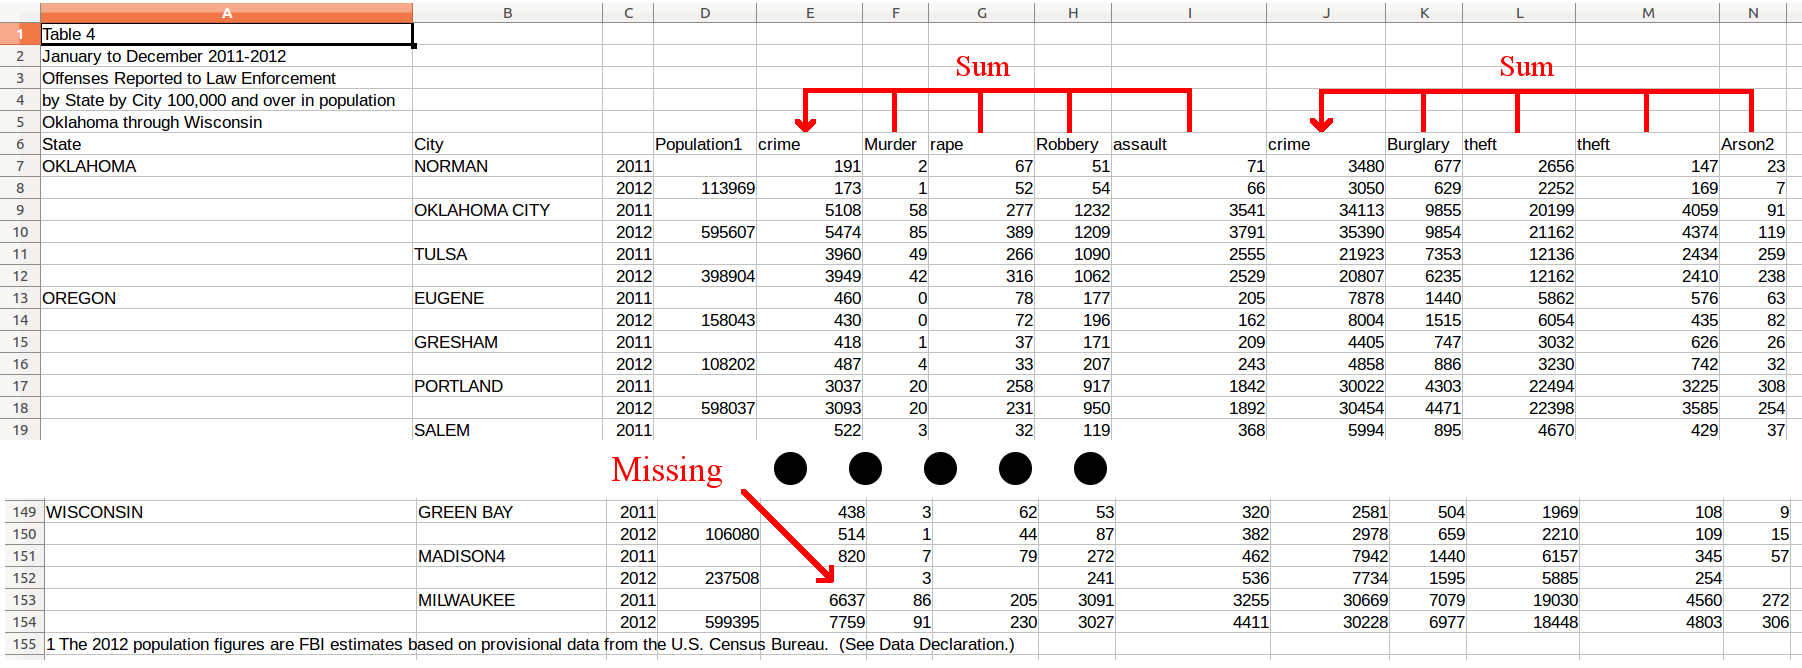
\includegraphics[width=\width]{figures/fbi_figure_highlighted.png}
%   \end{center}
%   \caption{Real world tabular constraint reconstruction: FBI crime statistics}
%   \label{fig:fbi}
%\end{subfigure}
% \hfill
% \begin{subfigure}{.29\textwidth}
\begin{center}
    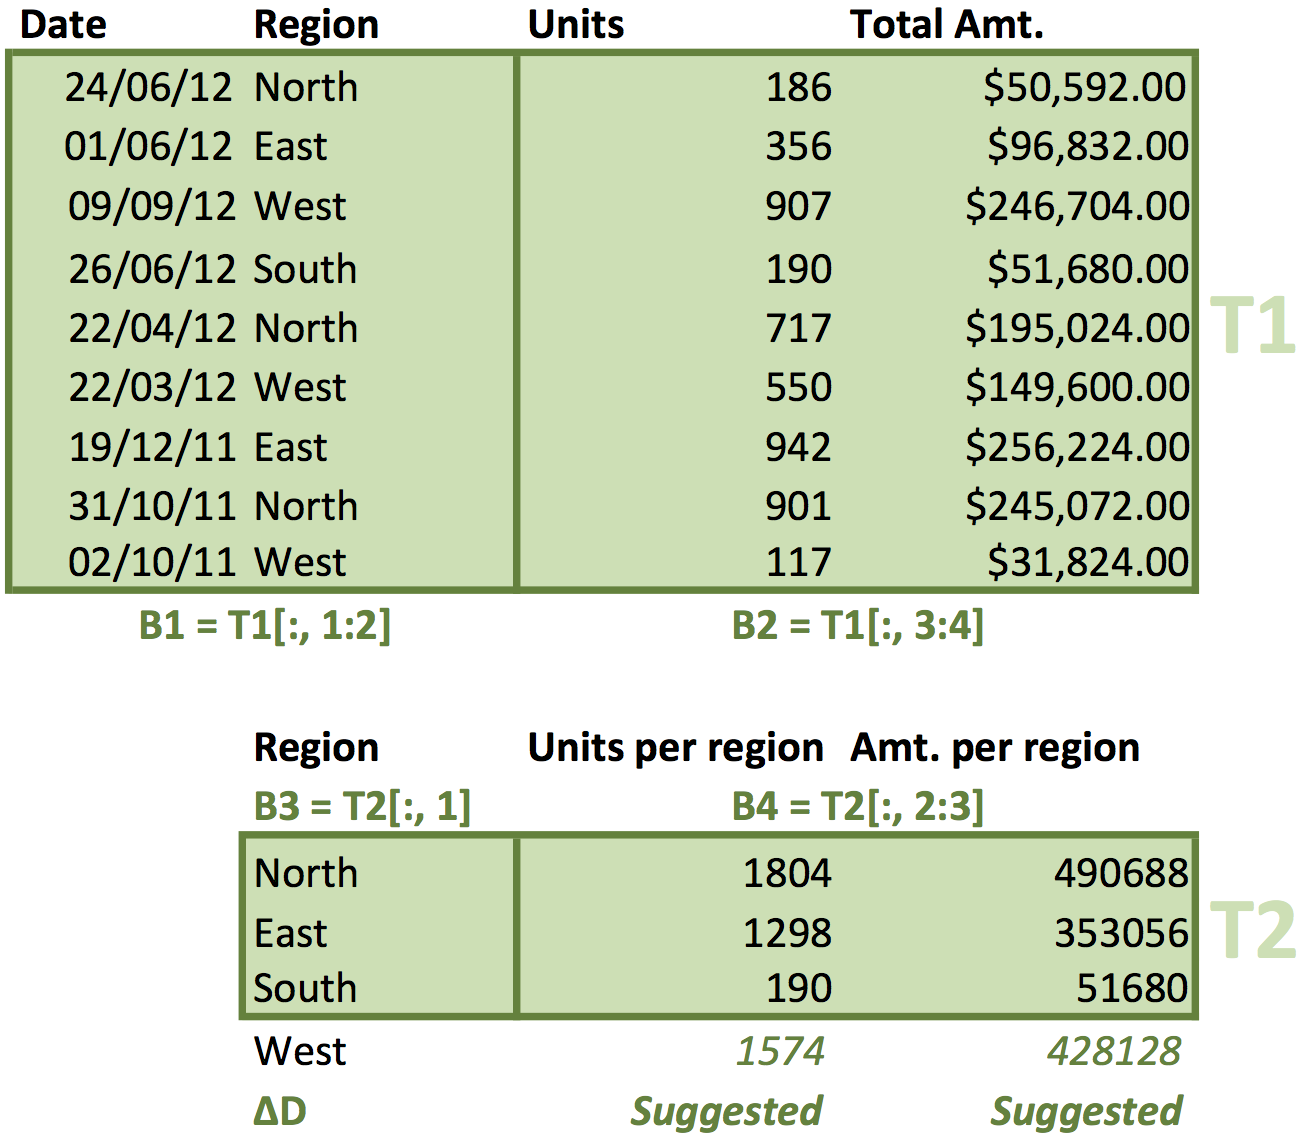
\includegraphics[width=1.0\linewidth]{figures/Learning.png}
  \end{center}
  \caption{Autocompletion works by learning constraint on a snapshot and combining those constraints with new data $\Delta D$.
  The figure shows how, given a new value \textit{West}, we can suggest values for the other cells in that row.}
  \label{fig:autocompletion_example}
%\end{subfigure}
\end{figure}

We consider two cases of error detection.
The first setting is the \textit{online} detection of errors and is similar to the autocompletion setting.
Using snapshots, we search for \textit{conflict} constraints, which are learned on a previous snapshot but do not agree with newly added data~$\Delta D$.
Such conflicts can indicate (typing) errors in the data just entered. For example, in case 'Wes' instead of 'West' was added in Figure~\ref{fig:autocompletion_example}.
%Conflict constraints can indicate errors in the input.
%However, such conflicts can be wrongly caused by spurious constraints.
%Hence, conflicts should perhaps only be detected if the snapshot data is large enough.
%An exact specification of what large enough means (i.e., how to measure the confidence in the constraint violation) is a separate application-dependent research question and will be investigated in the future work.

The second setting is \textit{offline} error detection in a static spreadsheet.
% Consider a use case concerning crime statistics provided by the FBI in Figure~\ref{fig:fbi}.
% Our system is able to detect the second sum constraint, however, a missing value prevents the first sum constraint from being learned.
% A possible approach to detect such missing or wrong values is to look at a sample of the table, e.g. trying to leave out each row, and compare the constraints learned on this sample with the constraints learned on the whole table.
  %The sample needs to be large enough such that we have enough confidence that the constraints are correct. For example, in Figure \ref{fig:fbi} all but one row satisfy the constraint, which is a strong indication that there is a constraint violation.
Instead of snapshots, one can repeatedly search for conflict constraints between the original spreadsheet and a sheet with a row or column removed. Many schemes can be devised for choosing which row(s) or column(s) are removed.
%This task can be formulated as online error detection by repeatedly partitioning the spreadsheet into a snapshot~$D_i$ and ``input'' $\Delta D_i$ (e.g. leave out each row and consider it as $\Delta D_i$) to detect conflicts.

%Of course, generating large enough samples and rows (columns) to be added can be done in multiple ways.
%In the limited case of detecting single errors one can leave out every row (column), consider the remaining data to be the sample and
%and the left out row (column) to be new input.

\section{Conclusions}\label{sec:conclusions}

% points: 1) can be a base for an actual plugin or a function in excel 2) novel problem and challenge for systems and constraint solvers 3) can be part of the complicated pipeline togehter with the header detection
Our goal is to automatically identify constraints in a spreadsheet.
We have presented and evaluated our approach, implemented as the system \sname, that is able to learn many different constraints in tabular data.
The resulting method has high recall, produces limited number of redundant constraints and is sufficiently efficient for normal and interactive use.

The approach is designed to find constraints that hold over entire columns and rows. In future work we plan to extend this to learn arbitrary nested constraints (e.g. $\sbl{r} = (\sbl{1} + \sbl{2}) / \sbl{3}$), as well as constraints over only a subset of the vectors. This may give rise to more redundant and spurious constraints, which was not problematic up to this point.

Two promising ways to mitigate redundant and spurious constraints are heuristic filtering or post-processing of the constraint set and the integration of our approach in an interactive setting where users can receive and provide feedback.
The latter is more similar to an active learning setting.

A final direction is that the current approach assumes noise-free data (but see the part on error correction); in inductive logic programming there has been much work on how to handle noisy data, while in constraint satisfaction a popular alternative is to consider \textit{soft} constraints that can be violated (at a cost). 
This could extend the approach to new application domains, beyond traditional spreadsheets.


\bibliographystyle{plain}
{
  \bibliography{references}}
\end{document}
